\documentclass[11pt]{article}

\usepackage[margin=1in]{geometry}
\usepackage[T1]{fontenc}
\usepackage{lmodern}
\usepackage{amsmath,amssymb,amsthm,booktabs,graphicx,array}
\usepackage{placeins}
\usepackage{microtype}
\usepackage{enumitem}
\usepackage{xurl}
\usepackage{caption}
\usepackage{hyperref}

\graphicspath{{figures/}}
\hypersetup{
  colorlinks=true,
  linkcolor=blue,
  citecolor=blue,
  urlcolor=blue,
  pdftitle={Structural Hawkes Ambiguity in Near-Critical Market Making},
  pdfauthor={Mayank Sharma and Rohit Kumar Mourya},
  pdfsubject={Robust market making under structural Hawkes ambiguity},
  pdfkeywords={Hawkes processes, robust market making, structural ambiguity, near-critical order flow, viscosity solutions, limit order books, queue-position risk}
}
\urlstyle{same}
\captionsetup{font=small,labelfont=bf}
\setlist[itemize]{topsep=2pt,itemsep=2pt,parsep=0pt}
\setlist[enumerate]{topsep=2pt,itemsep=2pt,parsep=0pt}
\setlength{\textfloatsep}{8pt plus 2pt minus 2pt}
\setlength{\floatsep}{8pt plus 2pt minus 2pt}
\setlength{\intextsep}{8pt plus 2pt minus 2pt}
\emergencystretch=1em
\makeatletter
\setlength{\@fptop}{0pt}
\setlength{\@fpsep}{8pt plus 2pt}
\setlength{\@fpbot}{0pt plus 1fil}
\makeatother

\newtheorem{theorem}{Theorem}
\newtheorem{proposition}{Proposition}
\newtheorem{assumption}{Assumption}
\newtheorem{remark}{Remark}

\newcommand{\E}{\mathbb{E}}
\newcommand{\R}{\mathbb{R}}
\newcommand{\cA}{\mathcal{A}}
\newcommand{\cU}{\mathcal{U}}
\newcommand{\Gammahat}{\widehat{\Gamma}}

\title{Structural Hawkes Ambiguity in Near-Critical Market Making}
\author{}
\date{}

\begin{document}
\begin{center}
{\LARGE\bfseries Structural Hawkes Ambiguity in Near-Critical Market Making\par}
\end{center}
\vspace{0.75em}

\begin{abstract}
This paper studies a narrow source of model risk in market making: uncertainty
about the self-excitation structure of Hawkes order flow. The structure is
encoded by a branching matrix $\Gamma$, while the distance to instability is
measured by the Perron root $\rho(\Gamma)$. In a reduced robust inventory model,
ambiguity in $\Gamma$ is amplified through the Hawkes resolvent
$(I-\Gamma)^{-1}$, so near-critical calibration error can become an economic
risk premium. The critical exponent depends on normalization: relative
critical-slack ambiguity gives a square-law reduced premium, while absolute
branching-matrix ambiguity contributes one additional derivative factor when
$\epsilon=o(1-\rho)$.

The paper gives a reduced-form spectral theorem and conditional robust-control
bridges under stated compact-PDMP, Lyapunov, weighted-comparison, and
smooth-interior assumptions. It then evaluates robust and nominal quoting
policies under common random numbers, Ogata event times, public LOBSTER sample
replays, Binance aggregate trades, and crypto order-book samples. The empirical
claim is deliberately limited: structural Hawkes ambiguity is visible in these
near-critical stress tests, but public Hawkes calibrations remain diagnostic
inputs rather than complete execution models.
\end{abstract}

\noindent\textbf{Authors.}
Mayank Sharma, Indian Institute of Technology Jodhpur, Department of
Engineering Science. Contact: \texttt{may1729int@gmail.com}.

Rohit Kumar Mourya, Indian Institute of Technology Jodhpur, Department of
Engineering Science. Contact: \texttt{rohitmourya1056@gmail.com}.

\medskip
\noindent\textbf{Status.}
Preprint / working paper.

\medskip
\noindent\textbf{Keywords.}
Hawkes processes; robust market making; structural ambiguity; near-critical
order flow; viscosity solutions; limit order books; queue-position risk.

\medskip
\noindent\textbf{AI disclosure.}
Generative AI tools assisted with language editing, LaTeX cleanup, code
scaffolding, experiment automation, validation-script review, and
reproducibility-package organization. The authors reviewed the outputs and
remain responsible for all mathematical claims, proofs, citations, code, data
processing, numerical experiments, and final text.

\medskip
\noindent\textbf{Reproducibility package.}
Code, tests, TeX sources, derived tables, and derived figures:
\href{https://github.com/mayank172900/mesa-sifin-reproducibility}{\texttt{github.com/mayank172900/mesa-sifin-reproducibility}}.

\section{Introduction}

When liquidity disappears during stress, the usual explanations are volatility,
inventory pressure, or lower fill probabilities. This paper focuses on a
smaller but sharper mechanism. If order flow is self-exciting and already close
to criticality, then uncertainty about the excitation structure can become
expensive by itself. The same estimation error in $\Gamma$ may be harmless far
from criticality and serious when $\rho(\Gamma)$ is close to one.

The contribution is narrow by design. Hawkes market making, robust market
making, near-critical Hawkes limits, and learned limit-order-book simulators
are all active areas. This paper studies their intersection:
structural Hawkes ambiguity in market making, the spectral amplification law it
creates, and reproducible diagnostics showing why near-critical Hawkes
calibrations should be stress-tested before being used inside a trading
simulator.

The paper makes four contributions. It identifies the resolvent channel through
which branching-matrix uncertainty amplifies risk-premium proxies. It separates
relative critical-slack ambiguity from absolute branching-matrix ambiguity,
which changes the critical exponent. It develops the reduced control problem
through a sequence of conditional finite-state, compact-PDMP, Lyapunov,
weighted-comparison, and interior-optimizer results. Finally, it reports
a reproducible experimental path from synthetic scaling tests to robust Bellman
policies, event-time execution
stress tests, public LOBSTER replays, Binance aggregate-trade diagnostics, and
crypto depth sanity checks.

\subsection*{Reader's map}

The main idea can be understood before reading the mathematical appendix that
follows the paper in the combined SSRN PDF. If order flow is described by a
Hawkes branching matrix $\Gamma$,
then the long-run effect of arrivals is filtered through the resolvent
$(I-\Gamma)^{-1}$. As $\rho(\Gamma)$ moves toward one, this resolvent grows in
the leading Perron direction. For a market maker uncertain about the excitation
matrix, this makes near-critical calibration error more than a small nuisance
parameter. It can be magnified into a meaningful economic risk.

The rest of the paper proceeds in three layers. The first is spectral and gives the
normalization-dependent amplification laws. The second is a robust-control
bridge showing how the spectral effect enters reduced Bellman/HJBI equations
for market making. The third is empirical and computational. The experiments do
not form a production execution engine. They ask whether the same risk layer
remains visible under finite-state policies, event-time simulation, public
LOBSTER replay, crypto clustering diagnostics, calibration noise, and ablation
tests.

\medskip
\noindent\fbox{\begin{minipage}{0.95\linewidth}
\textbf{Main claim.} MESA--market-making excitation-structure ambiguity--does
not claim that Hawkes models fully describe limit-order-book execution. It says
that, conditional on using a Hawkes structural layer, ambiguity in $\Gamma$ is
amplified near criticality, and the amplification exponent depends on how that
ambiguity is normalized. The theory establishes this reduced-form spectral
claim under stated assumptions; the experiments test whether the mechanism is
visible in the stress designs reported below.
\end{minipage}}

\section{Related Work and Positioning}

Nearby literatures approach this problem from several directions. Point-process
and Hawkes market-making models study weakly consistent LOB control
\cite{LawViens2019}, Hawkes impulse control \cite{Jain2025}, and adversarial or
reinforcement-learning variants \cite{WangHawkesARL2025}. A separate
LOB-simulation and forecasting literature uses neural Hawkes, multivariate
Hawkes, state-dependent Hawkes, and non-Hawkes realism-focused simulators to
improve realism and calibration
\cite{LalorSwishchuk2025,Kumar2024,Raffaelli2026,ElKarmiSimulator2025,Noble2026,Kimura2026}.
Recent work on robust quote refusal and latency-aware policies addresses
different forms of execution risk \cite{WangNoQuote2025,Jiang2025}. Empirical
Hawkes analyses also motivate concern about near-critical financial event flow
\cite{Hardiman2013}, while nearly unstable Hawkes limits clarify what happens
close to criticality \cite{SzymanskiXu2025,ElKarmi2026}. MESA is narrower than
these programs. Throughout the paper, MESA means market-making
excitation-structure ambiguity: a spectral ambiguity layer for Hawkes branching
matrices. It does not propose a new full LOB simulator or a competing RL agent;
it isolates how uncertainty in the branching matrix is amplified when the
Hawkes system is near instability.

\begin{table}[!htbp]
\centering
\scriptsize
\setlength{\tabcolsep}{2.5pt}
\renewcommand{\arraystretch}{0.82}
\resizebox{\linewidth}{!}{%
\begin{tabular}{@{}>{\raggedright\arraybackslash}p{5.0cm}cccc>{\raggedright\arraybackslash}p{5.8cm}@{}}
\toprule
Work & Hawkes MM & Robust MM & $\Gamma$ uncertainty & Near-critical scaling & MESA position \\
\midrule
Law--Viens 2019/2020 & no & no & no & no & Marked point-process/HJB-QVI LOB MM benchmark; MESA adds Hawkes branching-matrix ambiguity. \\
Wang--Ventre--Polukarov 2023/2025 quote/no-quote & no & yes & no & no & Robust quote-refusal/single-sided quoting benchmark; Hawkes branching uncertainty is outside its scope. \\
Wang--Ventre--Polukarov 2024/2025 Hawkes ARL & yes & yes & no & no & A close Hawkes/ARL policy benchmark; no branching-matrix ambiguity amplification law. \\
Jain et al. 2025 Hawkes impulse control & yes & no & no & no & A close HJB-QVI benchmark; robustness to $\Gamma$ is not the main object. \\
Lalor--Swishchuk 2025 neural Hawkes LOB & yes & no & no & no & Neural Hawkes LOB simulator/DRL market-making baseline; ambiguity amplification is complementary. \\
Kumar 2021/2024 Deep Hawkes & yes & no & no & no & Deep Hawkes high-frequency MM/simulation benchmark; MESA adds structural $\Gamma$ ambiguity diagnostics. \\
Guo--Lin--Huang 2023 Attn-LOB DRL \cite{GuoAttnLOB2023} & no & no & no & no & LOB-feature DRL baseline; focus is alpha learning rather than Hawkes structure. \\
Jiang et al. 2025 latency-aware RL & no & no & no & no & Latency/inventory-aware neural MM benchmark; robust Hawkes ambiguity is not modeled. \\
Raffaelli et al. 2026 multivariate Hawkes BTC LOB & no & no & no & no & Recent multivariate Hawkes BTC LOB calibration/forecasting study; robust control is outside its scope. \\
El Karmi 2025 deterministic Hawkes LOB simulator & no & no & no & no & Simulator-realism baseline with Hawkes-driven order flow; robustness is complementary. \\
Noble--Rosenbaum--Souilmi 2026 realism gap & no & no & no & no & Recent simulator-realism and execution-sensitivity study; MESA is a complementary risk layer. \\
Kimura 2026 state-dependent Hawkes & no & no & no & no & State-dependent Hawkes LOB with local supercriticality evidence; MESA targets robust $\Gamma$ ambiguity. \\
Szymanski--Xu 2025 nearly unstable Hawkes & no & no & no & yes & Near-critical Hawkes scaling limits; MESA adds market-making control and $\Gamma$-ambiguity premiums. \\
El Karmi 2026 bivariate nearly unstable Hawkes & no & no & no & yes & Recent bivariate near-critical Hawkes limit theory; MESA targets robust market-making premiums. \\
MESA reduced-form package & yes & yes & yes & yes & Reduced-form theorem, policy stress tests, and public-data calibration diagnostics. \\
\bottomrule
\end{tabular}}
\caption{Comparison with nearby work. The point is not to claim simulator
primacy, but to isolate the structural Hawkes ambiguity layer.}
\label{tab:sota}
\end{table}

The reproducibility package records the source URLs, visible code links, and
implementation notes used to construct the comparison. The intended position is
therefore modest: MESA is a spectral ambiguity-risk layer that can be attached
to richer simulators, not a substitute for them.

\FloatBarrier
\section{Model}

Let $N^{k,s}_t$ denote marked order arrivals by type $k$ and side $s$. The
exponential Hawkes intensity is
\[
\lambda^{k,s}_t = \mu^{k,s} +
\sum_{j,\sigma}\int_0^{t^-}
\alpha^{k,s}_{j,\sigma}\beta e^{-\beta(t-u)}\,dN^{j,\sigma}_u.
\]
Thus $\Gamma$ records the integrated excitation from each event type into each
other event type. Stability is governed by its Perron root: when
$\rho(\Gamma)<1$, the stationary mean intensity is
\[
\bar\lambda = (I-\Gamma)^{-1}\mu.
\]
This resolvent is the channel through which small errors in $\Gamma$ become
large near criticality.

A market maker chooses bid and ask offsets
$u_t=(\delta^b_t,\delta^a_t)\in\cU$ with inventory $q_t\in\{-Q,\ldots,Q\}$.
Nature chooses a structural model from an ambiguity set
\[
\cA_\epsilon = \{\Gamma\ge 0:
\|\Gamma-\Gammahat\|_F\le \epsilon,\ \rho(\Gamma)\le \rho_{\max}<1\}.
\]
The asymptotic statements are interpreted along Perron-regular local sequences
with $\rho_{\max}$ allowed to approach one, while numerical experiments use
finite stable stress scenarios below one. For absolute ambiguity, the derivative
law is local: if $\epsilon$ is not smaller than the remaining critical slack,
the perturbation can saturate at the stability cap and the simple
$(1-\rho)^{-3}$ expansion no longer applies.
For numerical work, this ambiguity set is discretized into the nominal matrix
and a small collection of Perron-aligned boundary perturbations.

\section{Theory and Main Results}

\begin{assumption}[Perron regularity]
$\Gamma$ is nonnegative, irreducible, and primitive, with Perron root
$\rho<1$. Let
$\mathrm{gap}(\Gamma)=\rho-\max_{j>1}|\lambda_j(\Gamma)|$.
Assume $\mathrm{gap}(\Gamma)\ge g_0>0$, the Perron root is simple, the Perron
eigenprojection $r\ell^\top$ is uniformly bounded under the normalization
$\ell^\top r=1$, and the reduced resolvent on the non-Perron spectral subspace
is uniformly bounded. This rules out non-Perron conditioning from carrying the
same singular order as the Perron pole.
\end{assumption}

\begin{proposition}[Resolvent amplification]
Under Perron regularity,
\[
(I-\Gamma)^{-1}
 =
\frac{r\ell^\top}{1-\rho(\Gamma)} + O(1/\mathrm{gap}).
\]
Consequently, price-risk loadings whose Perron projection is bounded away from
zero on the Perron-regular class are exposed to the same leading near-critical
blow-up.
\end{proposition}

\begin{proposition}[Perturbation direction]
For a small perturbation $E$,
\[
\rho(\Gamma+E)-\rho(\Gamma)
 =
\ell^\top E r + O(\|E\|_F^2/\mathrm{gap}).
\]
The first-order Frobenius direction that maximally increases the Perron root is
$E^\star=\ell r^\top/\|\ell r^\top\|_F$, distinct from the resolvent projection
$r\ell^\top$.
\end{proposition}

\begin{theorem}[Reduced-form normalization-dependent ambiguity premium]
Suppose the robust half-spread correction is locally linear in an effective
Hawkes variance proxy proportional to $(1-\rho)^{-2}$. The square-law exponent
uses this normalized-throughput/resolvent-squared risk proxy; alternative raw
count-variance conventions may change the baseline exponent, but not the
distinction between relative-slack and absolute-$\Gamma$ ambiguity. Then relative
critical-slack
ambiguity, $\Delta\rho=O(\epsilon_{\mathrm{rel}}(1-\rho))$, gives
\[
\psi = O\!\left(\frac{\epsilon_{\mathrm{rel}}}{(1-\rho)^2}\right).
\]
Absolute branching-matrix ambiguity, $\Delta\rho=O(\epsilon)$ with
$\epsilon=o(1-\rho)$, gives the more singular derivative law
\[
\psi = O\!\left(\frac{\epsilon}{(1-\rho)^3}\right).
\]
Matching lower bounds require Perron-visible loadings, a feasible
Perron-aligned perturbation, an active worst-case selector, and an interior
quote regime before spread caps or no-quote constraints bind.
\end{theorem}

\begin{remark}
The theorem is stated at the reduced-form level because the amplification
mechanism is spectral, while the market-making problem can be embedded in
several control formulations. The mathematical appendix gives scalar and
finite-dimensional Perron-visible versions of the bridge, a finite-state
Bellman verification theorem, and a compact continuous-intensity HJBI
verification theorem for a truncated multitype Hawkes control game. It also
records the Lyapunov, weighted-comparison, and local differentiability
arguments used to connect the reduced premium calculation to smooth interior
quote optimizers. The main limitations are active-set changes from no-quote or
spread caps, the compact-PDMP comparison hypotheses, and extensions to
state-dependent, power-law, or learned Hawkes kernels.
\end{remark}

\section{Computational Design}

The empirical design combines complementary simulations, control solvers, and
replay diagnostics. Its roles are to test the predicted critical scaling,
evaluate robust quote policies under controlled Hawkes variation, and compare
the resulting behavior with public limit-order-book data. The components are:

\begin{enumerate}[nosep]
\item Scaling diagnostics for scalar and multitype resolvent proxies.
\item Common-random-number policy evaluation under full simulated Hawkes paths.
\item A finite-scenario robust inventory Bellman solver for a scalar reduced
state with side-level quote/no-quote actions.
\item A reduced event-queue backtest on Ogata event times with queue-ahead
mechanics and no-quote side-time accounting.
\item Displayed-depth, residual-volume priority-aware level-10, and
deepest-public level-50 LOBSTER replays on public message/order-book streams.
\item Observable level-10 order-book reconstruction from messages, checked
against official LOBSTER snapshots.
\item Ogata-thinning validation and time-step bias diagnostics.
\item LOBSTER Hawkes diagnostics over event type, time scale, marks, and side
labels.
\item Binance aggregate-trade event diagnostics for public crypto clustering.
\end{enumerate}

The Bellman recursion uses side-specific quote/no-quote controls: on each side
the market maker either posts at a chosen offset or withdraws liquidity.
\begin{align*}
h_n(q)=\max_{a^b,\delta^b,a^a,\delta^a}\min_{\Gamma\in S}\Big\{&
-\Delta t\left(\phi q^2+\frac{\gamma}{2}\sigma^2(\Gamma)q^2\right)\\
&+p_b(\delta^b+h_{n+1}(q+1))
+p_a(\delta^a+h_{n+1}(q-1))\\
&+(1-p_b-p_a)h_{n+1}(q)\Big\}.
\end{align*}
The indicators $a^b,a^a\in\{0,1\}$ encode side activity; when a side is
inactive, its fill probability is set to zero.

\begin{theorem}[Finite-state Bellman verification]
Consider a finite state space encoding inventory and Hawkes regimes, a nonempty
finite quote/no-quote action set at each state, a conservative finite-state
generator $L^{u,\Gamma}$, bounded rewards, bounded terminal payoff, and a
finite rectangular ambiguity set $S$ of stable branching matrices. The
finite-regime robust control problem has the max--min value. In continuous time
its value is the unique bounded solution of the finite-state HJBI ODE
\[
-\partial_t V(t,x)=
\max_{u\in U(x)}\min_{\Gamma\in S}
\left\{r(x,u,\Gamma)+\sum_y L^{u,\Gamma}(x,y)V(t,y)\right\},
\qquad V(T,x)=g(x),
\]
On a time grid, the analogous backward Bellman recursion is exact for the
chosen stochastic one-step kernel, and for an explicit Euler kernel requires
$\Delta t$ small enough that $I+\Delta t L^{u,\Gamma}$ is stochastic.
Deterministic Markov selectors attain the finite max--min. This identifies
the finite-scenario quote/no-quote dynamic program with a discretized robust
finite-state game. The continuous-intensity Hawkes HJBI is
not covered by this finite-state argument; the compactness, Lyapunov, and
weighted-comparison results below supply the bridge to that setting.
\end{theorem}

\begin{theorem}[Conditional compact continuous-intensity HJBI verification]
Consider the truncated multitype Hawkes control state
$X_t=(q_t,\lambda_t)$, with finite inventory
$q_t\in\{-Q,\ldots,Q\}$ and compact intensity domain
$\lambda_t\in K\subset\R_+^d$. Between jumps,
$d\lambda_t=\beta(\mu-\lambda_t)\,dt$, and a mark-$i$ jump maps
$\lambda$ to $\Pi_K(\lambda+\beta\Gamma e_i)$, where $\Pi_K$ is a fixed
Lipschitz truncation map into $K$. Suppose the quote action set
and the rectangular ambiguity set $\mathcal A$ are compact, all rewards,
terminal payoffs, and controlled mark intensities are bounded and continuous,
the rates and jump maps are uniformly Lipschitz on each inventory slice,
$\sup_{\Gamma\in\mathcal A}\rho(\Gamma)<1$, and the compact PDMP game satisfies
the standard dynamic-programming and bounded-comparison principles for the
rectangular admissible class, using standard PDMP, stochastic-control, and
viscosity-solution machinery
\cite{Davis1993,FlemingSoner2006,CrandallIshiiLions1992}. Then the robust market-making game has a bounded
uniformly continuous value function, and it is the unique bounded viscosity
solution of
\[
-\partial_t V=
\sup_{u}\inf_{\Gamma\in\mathcal A}
\left\{
r(q,\lambda,u,\Gamma)+\mathcal L^{u,\Gamma}V(q,\lambda)
\right\},\qquad
V(T,q,\lambda)=g(q,\lambda),
\]
where $\mathcal L^{u,\Gamma}$ is the Hawkes PDMP generator. If the value is
classically differentiable and the Hamiltonian has measurable saddle
selectors, those selectors verify the robust value. Consequently, the truncated
continuous-intensity game admits the claimed HJBI characterization under the
stated compact-PDMP hypotheses. Passing to the global, untruncated
near-critical model still requires the stability and comparison arguments
developed next.
\end{theorem}

\begin{theorem}[Conditional untruncated Hawkes Lyapunov bridge]
For the unprojected Hawkes intensity state $\lambda_t\in\R_+^d$, suppose there
exist $v>0$ and $\kappa>0$ such that
$\Gamma^\top v\le(1-\kappa)v$ for every
$\Gamma\in\mathcal A$, fix $p>1$, and suppose controlled mark rates satisfy
$0\le\Lambda_i(q,\lambda,u,\Gamma)\le \lambda_i$. Then
$W_v(\lambda)=1+v^\top\lambda$ satisfies a uniform Foster--Lyapunov drift,
\[
\mathcal L^{u,\Gamma}W_v(q,\lambda)
\le C_0-C_1W_v(\lambda),
\]
and, after changing constants, the standard polynomial-weight version
\[
\mathcal L^{u,\Gamma}W_v(\lambda)^p
\le C_{0,p}-C_{1,p}W_v(\lambda)^p.
\]
Hence the untruncated controlled Hawkes PDMP is nonexplosive and has finite
$p$th weighted maximal moments on finite horizons. For rewards and terminal
payoffs with at most linear $W_v$-growth, compact truncations $\{W_v\le R\}$
have exit probability at most $C_{T,p}W_v(\lambda)^p/R^p$, and the payoff
tail error is of order $R^{1-p}$. Thus the compact projection is not needed for
stability or tightness. What remains is uniqueness of the limiting HJBI on the
unbounded intensity domain, addressed by the weighted comparison result below.
\end{theorem}

\begin{theorem}[Sufficient weighted-comparison bridge for the untruncated HJBI]
Following the standard weighted-barrier and doubling-of-variables logic used in
viscosity comparison arguments
\cite{CrandallIshiiLions1992,FlemingSoner2006}, assume common Lyapunov
subcriticality, compact ambiguity, and either a fixed
compact control set or a compact control correspondence continuous in Hausdorff
distance, continuous locally Lipschitz controlled rates with
$0\le\Lambda_i\le\lambda_i$, Lipschitz affine Hawkes jump maps, linearly
growing rewards, and the weighted boundary condition
\[
\limsup_{R\to\infty}
\sup_{\substack{t\in[0,T],\,q\in\{-Q,\ldots,Q\}\\ W_v(\lambda)\ge R}}
\frac{U(t,q,\lambda)-V(t,q,\lambda)}{W_v(\lambda)}\le 0
\]
for every subsolution $U$ and supersolution $V$ being compared. Then any
upper-semicontinuous weighted-growth subsolution of the untruncated HJBI is
dominated by any lower-semicontinuous weighted-growth supersolution with larger
terminal data. Hence, within any $W_v$-weighted subclass with a fixed boundary
condition at infinity, the untruncated robust Hawkes control value is the
unique viscosity solution, and compact truncation solutions converge to it
locally uniformly.
\end{theorem}

\begin{theorem}[Interior robust quote optimizer sensitivity]
Fix the state and adjoint variables in the HJBI Hamiltonian, and let $\theta$
parameterize either the branching matrix or the center of the ambiguity set.
Suppose that, near $(\delta_0,\theta_0)$, the robust reduced Hamiltonian
$\mathfrak H(\delta,\theta)=\inf_{\Gamma'\in\mathcal A(\theta)}
\mathcal H(\delta,\Gamma')$ has a unique $C^1$ active worst-case selector, the
quote constraints are inactive, $\mathfrak H$ is $C^2$ in $\delta$ with
continuous mixed derivative $D^2_{\delta\theta}\mathfrak H$, $\delta_0$ is the
unique local maximizer at $\theta_0$, and
$D^2_{\delta\delta}\mathfrak H\preceq -mI$ locally. Then, for $\theta$ near
$\theta_0$, there is a unique interior quote maximizer $\delta^*(\theta)$ in
the corresponding quote neighborhood, and the map $\theta\mapsto\delta^*(\theta)$
is locally $C^1$ with
\[
D_\theta\delta^*(\theta_0)=
-\left[D^2_{\delta\delta}\mathfrak H(\delta_0,\theta_0)\right]^{-1}
D^2_{\delta\theta}\mathfrak H(\delta_0,\theta_0).
\]
In the one-dimensional half-spread case, if $e$ is a Perron-adverse structural
direction and the directional mixed derivative in direction $e$ is nonnegative,
then the robust interior half-spread widens to first order. No-quote
boundaries, spread caps, and changes in the active adversary fall outside this
smooth interior calculation and instead require active-set analysis.
\end{theorem}

The computations use vectorized quote-grid evaluation and scenario-level
parallelism. To make policy comparisons attributable to the policy rather than
simulation noise, paired evaluations use fixed seeds and common random numbers.

\section{Experiments}

We first test the critical-scaling predictions in controlled ablations, then
evaluate the robust quote policies in simulated and replayed order-flow
environments. The experiments are ordered from mechanism-level checks to
market-data diagnostics.

\subsection{Scaling Ablations}

\begin{table}[!htbp]
\centering
\begin{tabular}{@{}llr@{}}
\toprule
Object & Family & Mean slope \\
\midrule
Relative-slack premium & scalar & -2.000 \\
Absolute-Gamma derivative & scalar & -3.000 \\
Matrix resolvent & rank1 & -3.191 \\
Matrix resolvent & block & -3.213 \\
Matrix resolvent & near-degenerate & -3.202 \\
Matrix resolvent & sparse & -3.283 \\
\bottomrule
\end{tabular}
\caption{Critical exponent ablation. Relative critical-slack ambiguity and
absolute branching-matrix ambiguity produce the distinct blow-up rates
predicted by the reduced-form theory.}
\end{table}

\begin{figure}[!htbp]
\centering
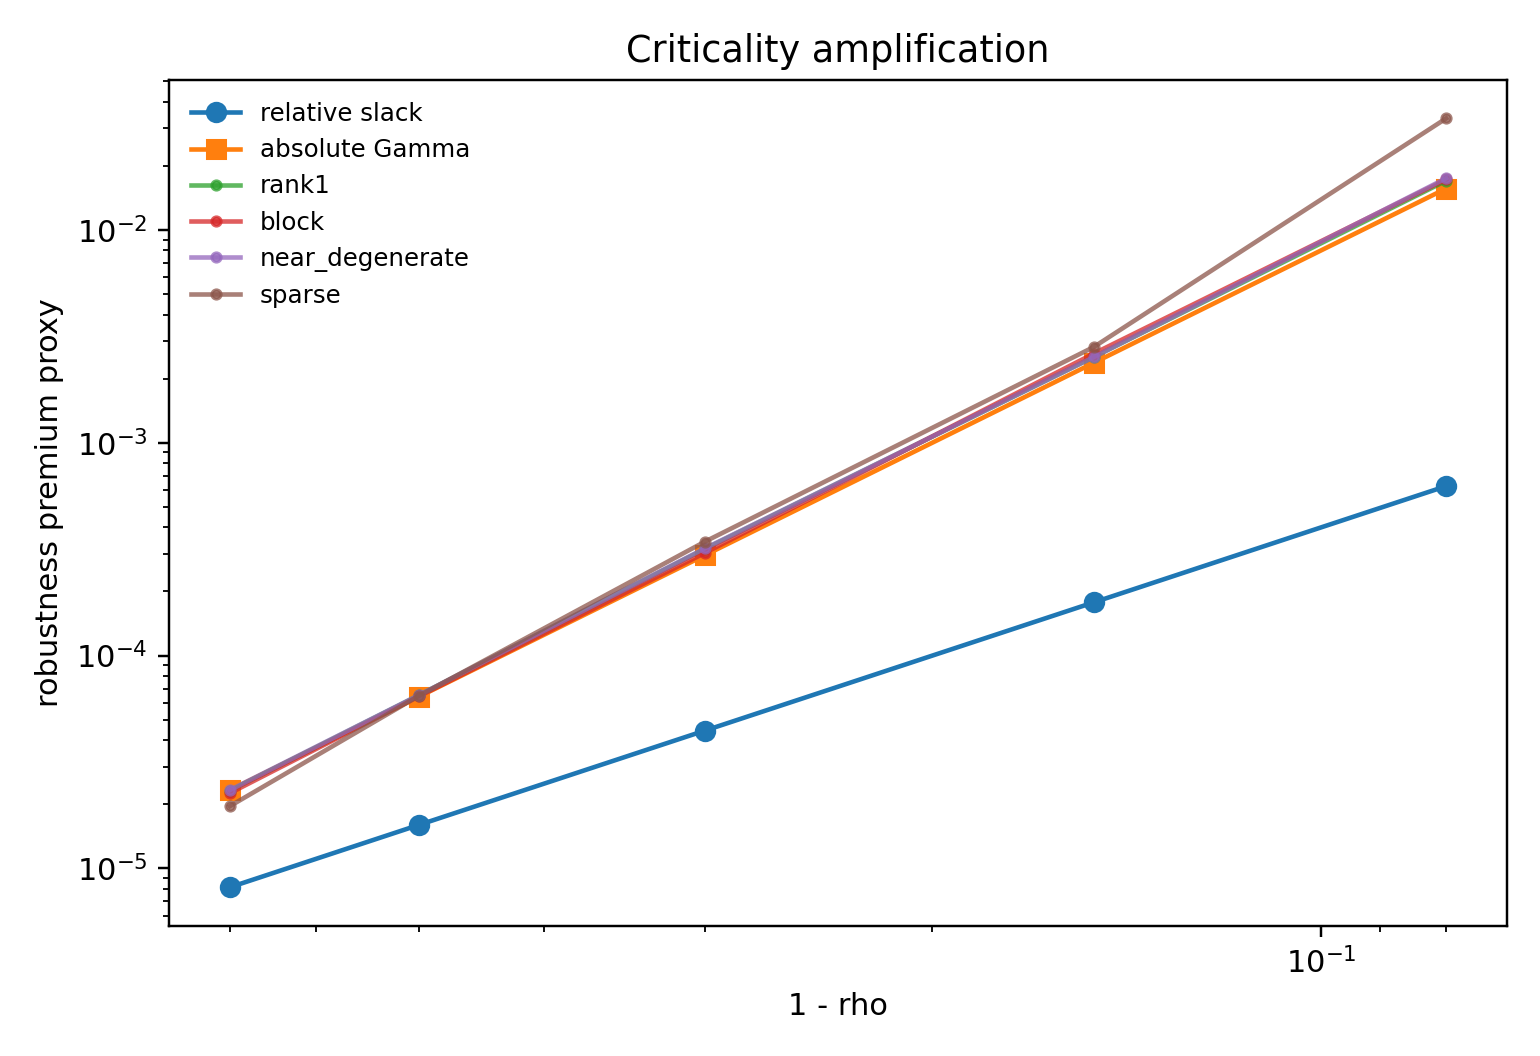
\includegraphics[width=.72\linewidth]{figures/criticality_scaling.png}
\caption{Criticality amplification under relative-slack ambiguity,
absolute-$\Gamma$ perturbations, and matrix-resolvent stress designs.}
\end{figure}

To separate the exponent from the particular stress design, we use a targeted
spectral-gap and visibility ablation based on a two-mode branching matrix with
eigenvalues $\rho$ and $1-k(1-\rho)$ for $k\in\{2,4,8\}$. When the payoff
loading is Perron-visible and the ambiguity set is aligned with the Perron
direction, the estimated slope is $-2.00$, with median normalized premium ratio
$2.8125$. A weakly Perron-visible loading recovers the same exponent after
visibility normalization. By contrast, a Perron orthogonal loading has no
positive Perron-aligned premium. When the adversary is instead allowed to move
the second eigenmode, the orthogonal loading again has slope $-2.00$ as that
mode approaches criticality. For weakly visible loadings, however, the median
normalized second-mode coefficient falls from $2.639$ at $k=2$ to $0.0365$ at
$k=8$. The lower-bound statement therefore requires both Perron visibility and
an ambiguity set that activates the Perron direction; otherwise the leading
coefficient can vanish or be transferred to another near-critical mode.

\begin{figure}[!htbp]
\centering
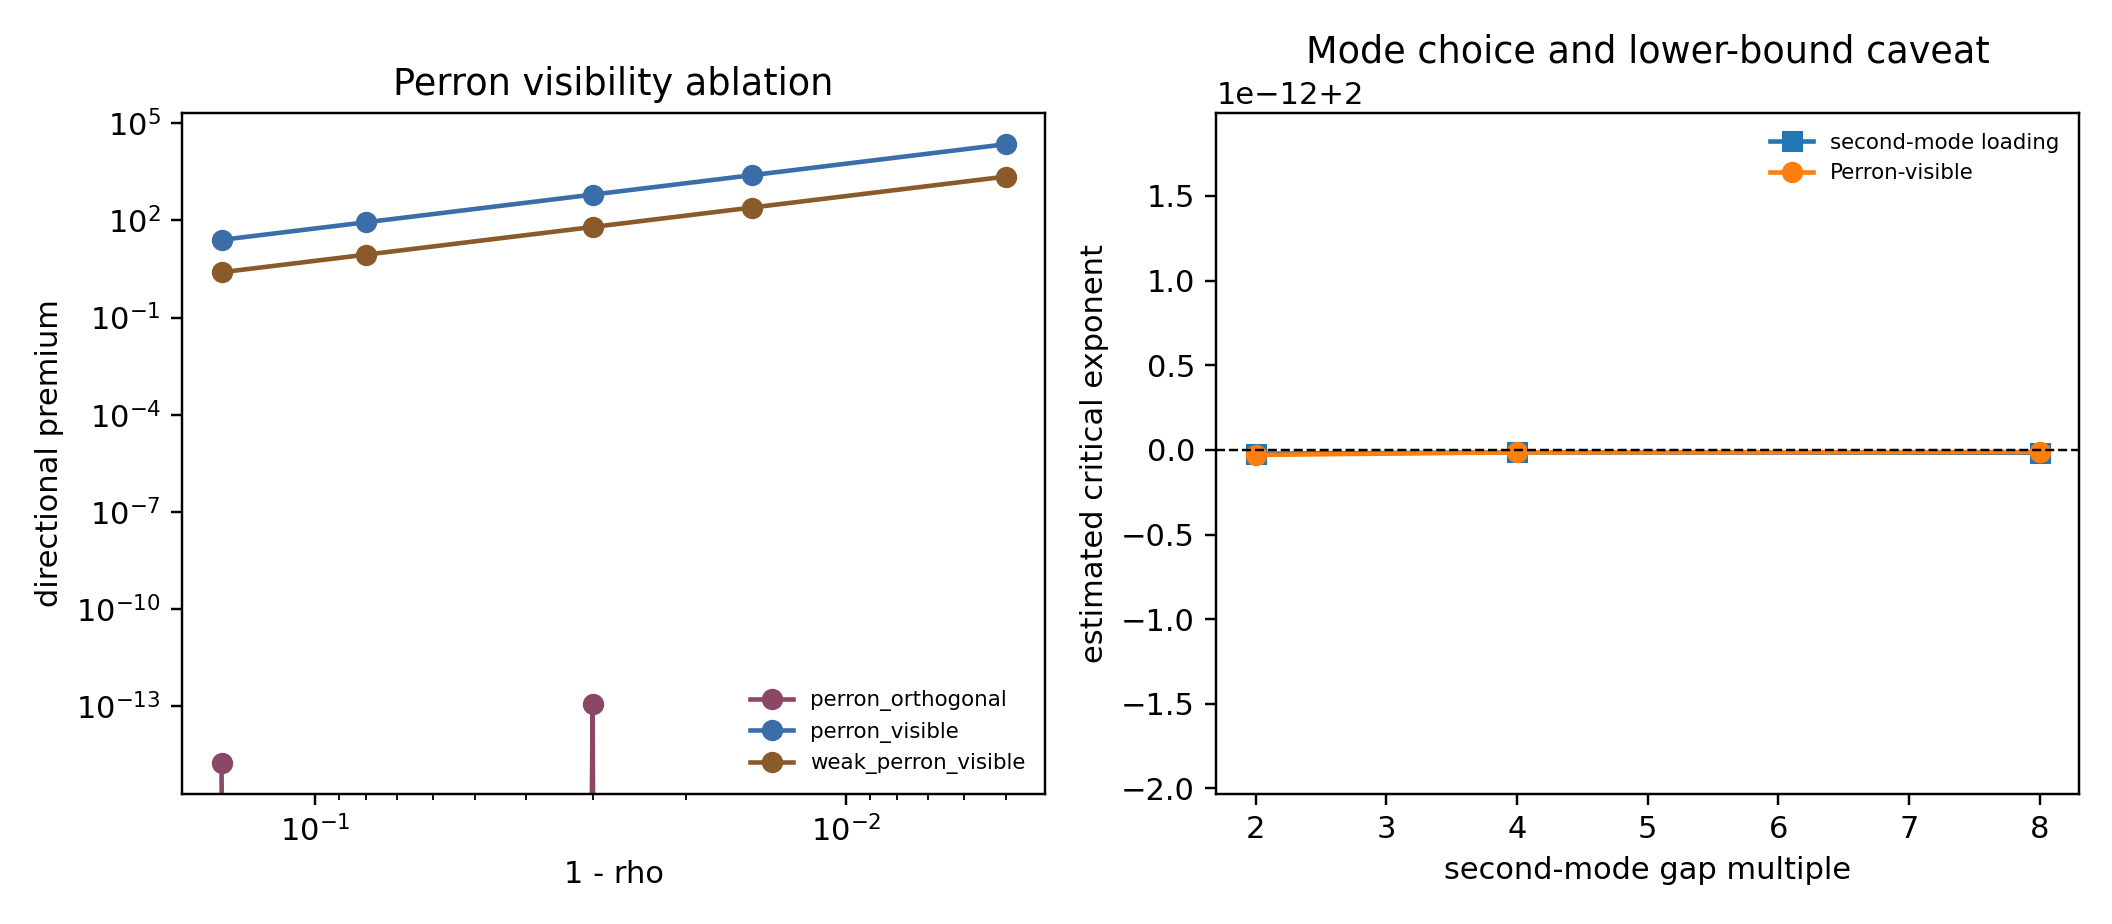
\includegraphics[width=.76\linewidth]{figures/spectral_gap_ablation.png}
\caption{Spectral-gap and Perron-visibility ablation. Perron-visible loadings
recover the square law under aligned ambiguity, while orthogonal loadings only
respond to second-mode perturbations.}
\end{figure}

\FloatBarrier
\subsection{Policy Ablations}

\begin{table}[!htbp]
\centering
\scriptsize
\resizebox{\linewidth}{!}{%
\begin{tabular}{@{}lrrr>{\raggedright\arraybackslash}p{2.7cm}@{}}
\toprule
Policy & Certainty equivalent & CVaR5 & Mean diff vs nominal & Paired 95\% CI \\
\midrule
robust\_gamma & -13.944 & -38.073 & 0.012 & [0.005, 0.020] \\
robust\_vol\_only & -13.956 & -38.087 & 0.000 & [0.000, 0.000] \\
nominal\_hawkes & -13.956 & -38.087 & baseline & -- \\
robust\_gamma\_abs & -13.624 & -37.321 & 0.306 & [0.257, 0.359] \\
known\_true\_gamma\_no\_ambiguity & -13.952 & -38.082 & 0.004 & [-0.002, 0.011] \\
as\_poisson & -13.974 & -38.113 & -0.017 & [-0.026, -0.008] \\
liquidity\_guard & -13.624 & -37.321 & 0.306 & [0.256, 0.355] \\
\bottomrule
\end{tabular}}
\caption{Common-random-number policy ablation.}
\end{table}

The intervals are paired bootstrap intervals over common-random-number paths,
so each policy is compared with nominal on the same simulated realizations. In
the main ablation, the absolute-Gamma and liquidity-guard policies have the
highest reported certainty equivalents, CVaR5 values, and paired mean-wealth
differences.
The relative-slack robust-Gamma policy is closer to nominal, with a smaller but
positive paired mean-wealth difference. We do not interpret the
known-true-$\Gamma$ benchmark as an oracle optimum: it is given the stressed
$\rho$, but it does not carry an ambiguity premium, so it under-hedges model
risk in this stress design. The table is best read as evidence that the policy
response depends materially on the ambiguity normalization and on the
withdrawal rule.

\FloatBarrier
\subsection{Policy Time-Step Audit}

The simulator validation below shows that near-critical Hawkes counts can be
sensitive to bin width, so we repeat the focused policy comparison at
$\Delta t\in\{0.04,0.02,0.01\}$ for the stressed $\epsilon=0.02$,
$\hat\rho=0.92$ scenario. Across the tested time steps, the relative-slack
robust-Gamma policy keeps a positive mean-wealth advantage over nominal Hawkes:
$0.042$--$0.060$. The absolute-Gamma policy produces much larger mean-wealth
gains, $1.154$--$1.366$, but with negative lower paired 5\% quantiles,
consistent with the broader point that ambiguity normalization changes the
economic policy, not only the scale of the premium.

\begin{figure}[!htbp]
\centering
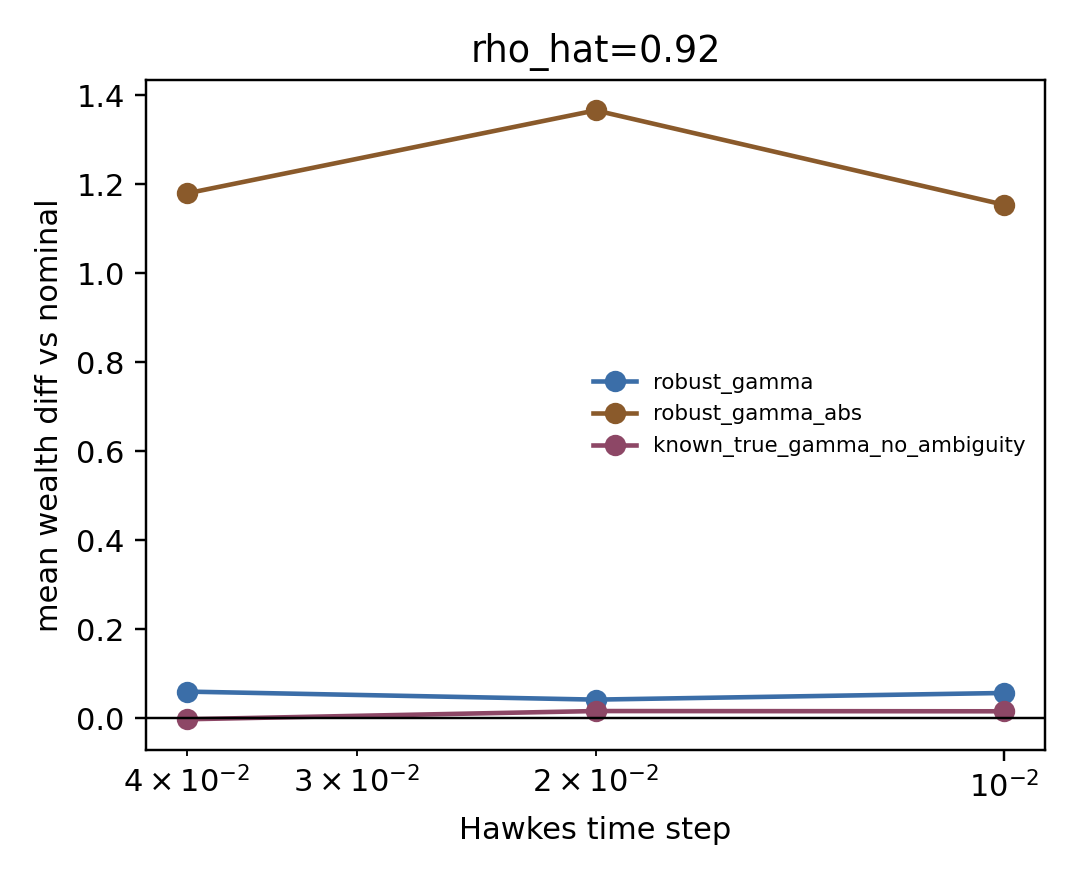
\includegraphics[width=.62\linewidth]{figures/policy_dt_convergence.png}
\caption{Focused policy time-step check. Positive values mean the policy
outperforms nominal Hawkes on the same scenario.}
\end{figure}

\FloatBarrier
\subsection{Ogata Arrival Audit}

We next compare the fast binned Hawkes recursion with event times generated by
Ogata thinning and then binned onto the same decision grid. In the
$\epsilon=0.02$, $\hat\rho=0.92$ check, the discrete recursion produces more
events than the Ogata reference: mean total events are $226.8$ under the
discrete recursion and $185.5$ under Ogata-binned arrivals. The relative-slack
robust-Gamma policy is positive relative to nominal under discrete arrivals,
with mean-wealth advantage $0.030$, but is essentially flat and slightly
negative under Ogata-binned arrivals, with mean-wealth difference $-0.001$ and
paired 5/95 quantiles $0.002$ and $0.049$, reflecting a small number of negative
tail paths. Absolute-Gamma is positive under both generators, with advantages
$0.705$ and $0.690$ and paired 5/95 quantile ranges roughly
$[-0.527,2.651]$ and $[-0.524,2.598]$. This check weakens any blanket claim that robust-Gamma dominates under
every arrival generator, and it shows that the relative-slack result is
generator-sensitive even though the absolute-Gamma result is similar across the
two generators.

\begin{figure}[!htbp]
\centering
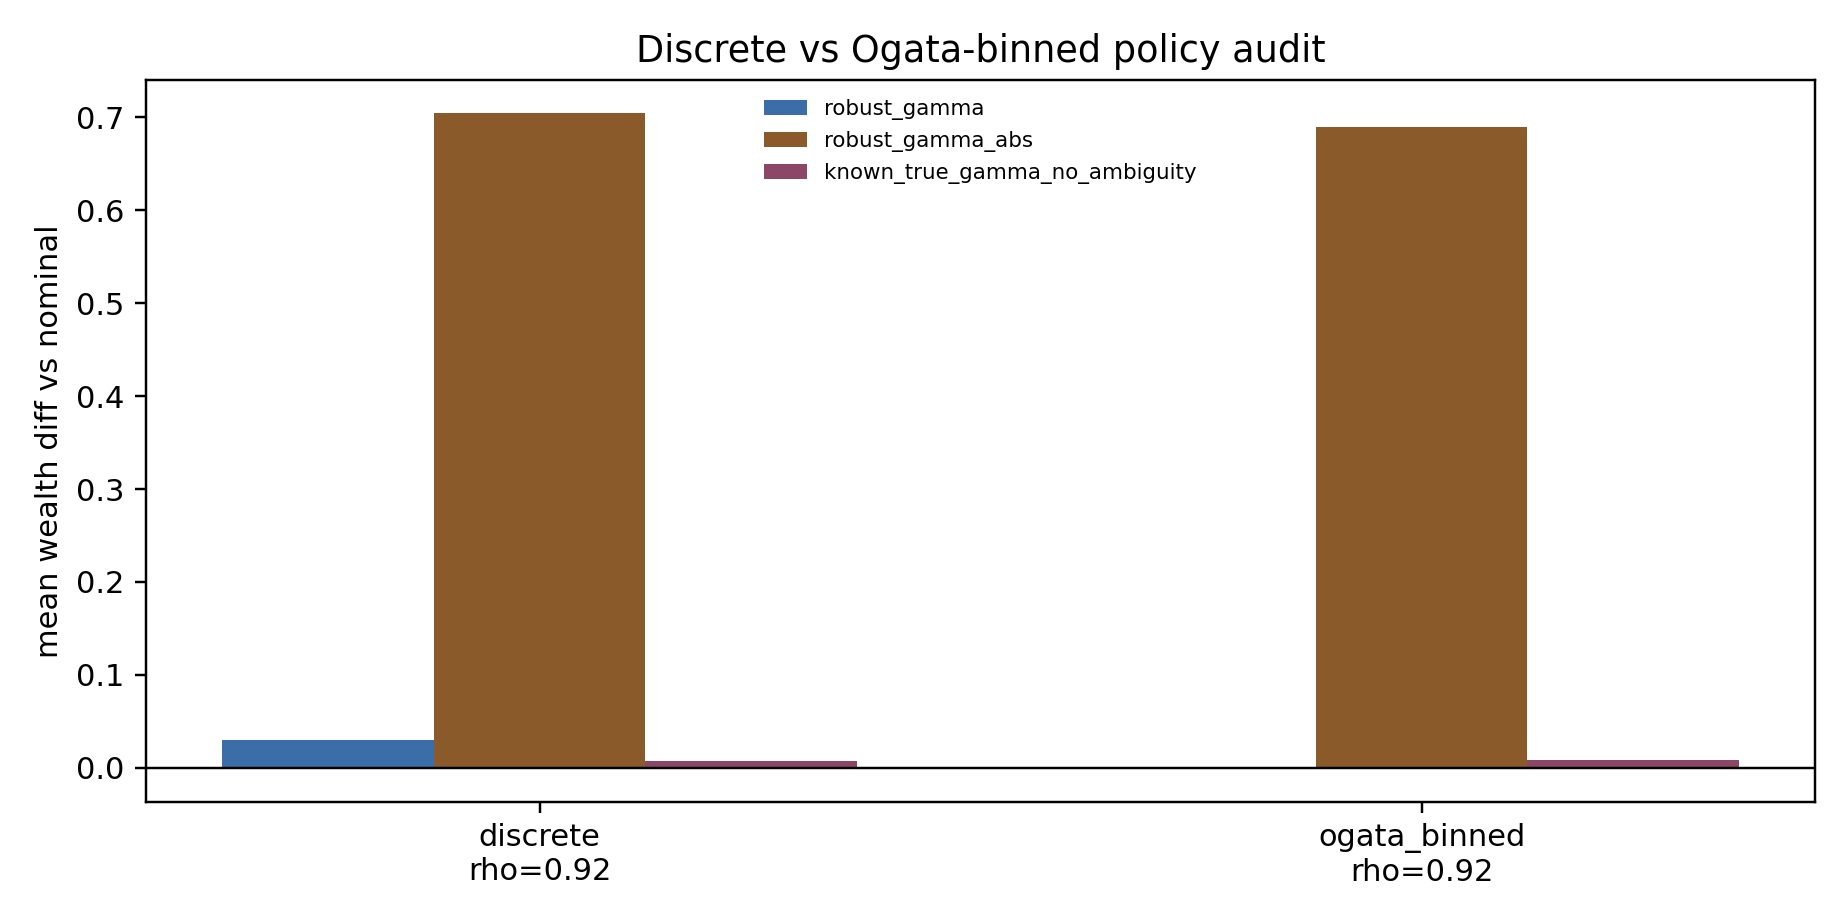
\includegraphics[width=.62\linewidth]{figures/policy_ogata_audit.png}
\caption{Focused policy check under fast discrete arrivals and Ogata-binned
event arrivals for $\hat\rho=0.92$.}
\end{figure}

\FloatBarrier
\subsection{Event-Queue Backtest}

Finally, we run a reduced event-driven queue backtest on Ogata Hawkes event
times. The evaluator holds the event path fixed across policies, updates quotes
every $\Delta t=0.02$, tracks a simple queue-ahead state, and records the
side-time spent not quoting. For $\hat\rho=0.92$ over 24 paths, robust-Gamma is
nearly flat but positive relative to nominal, with mean-wealth difference
$0.0125$ and paired 5/95 quantiles $[0.004,0.025]$, while absolute-Gamma and the
liquidity guard each improve mean wealth by $0.342$ with paired 5/95 quantiles
$[0.115,0.687]$. In this reduced run, fill rates are identical across policies at
$0.943$, the side-time no-quote fraction is $0.064$, and the full no-quote time
fraction is zero. This is not a production queue simulator, but it does provide
an event-time execution stress test for the checked regime.

\begin{figure}[!htbp]
\centering
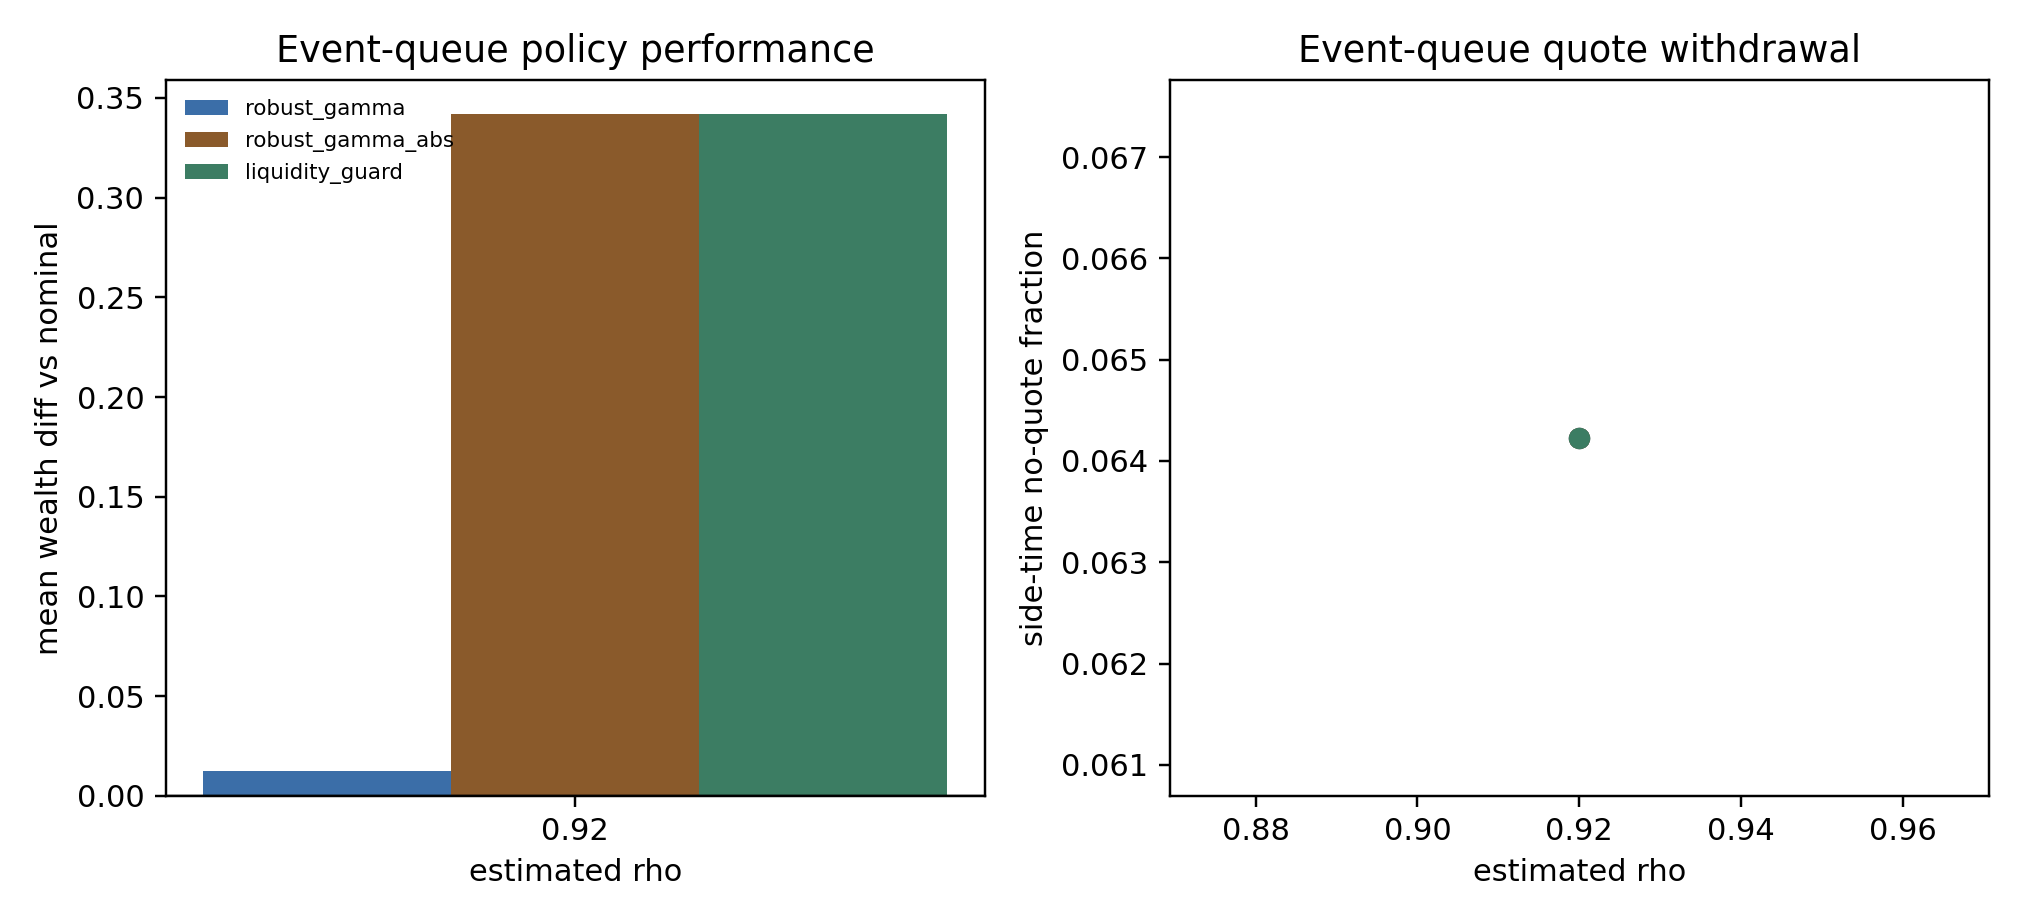
\includegraphics[width=.76\linewidth]{figures/event_queue_backtest.png}
\caption{Reduced event-queue performance and shared side-time no-quote fraction.}
\end{figure}

\FloatBarrier
\subsection{Public LOBSTER Top-Of-Book Replay}

The first replay asks whether the policy regimes observed in simulation also
appear when replayed on public LOBSTER message/order-book streams. The replay
uses up to the first 80,000 synchronized messages per ticker, posts active policies at
the displayed L1 quotes subject to an inventory cap, depletes a simple
queue-ahead proxy using observed execution sizes, and marks to the observed
midprice. Under the calibrated side-aware spectral radii, all tested policies
remain inside the L1 activity threshold, so the replay does not force an
artificial separation: mean terminal wealth is $341.691$, mean fills are
$3071.8$, and side-time no-quote share is $0.198$ for each policy. Under the
near-critical stress setting $\hat\rho=0.97$, nominal and relative-slack
robust-Gamma remain active on the same real event streams, while absolute-Gamma
and the liquidity guard fully withdraw: their mean wealth difference versus
nominal is $-341.691$, mean fills are zero, and side-time no-quote share is
one. This should not be read as a production queue simulator. Its narrower
point is that the quote-withdrawal transition appears in this public replay
when the same policies are placed on observed L1 event paths and prices.

The next replay keeps the L1 restriction but makes quote placement visible.
Each continuous policy offset is rounded into one of four displayed states:
join the best quote, improve inside the spread, rest away from L1, or withdraw.
Away quotes are not filled, because one-level data cannot identify hidden
depth. Under calibrated side-aware spectral radii, tick rounding still makes
policy PnL values coincide, but the state mix explains where the quotes would have
gone: mean side-time is $0.024$ joining, $0.428$ improving, $0.448$ away from
L1, and $0.101$ withdrawn. Under $\hat\rho=0.97$, absolute-Gamma and the
liquidity guard fully withdraw. This is a more informative public-data check
than the binary replay, while still stopping short of production execution
claims.

We then let away quotes interact with displayed depth by replaying the uniform
level-10 LOBSTER panel. If a rounded quote rests inside the displayed ten-level
ladder, the replay initializes queue-ahead from all better displayed levels
plus a same-level queue fraction; observed executions and visible depth changes
can then deplete that queue. Under calibrated side-aware spectral radii,
policies still coincide after tick rounding, but the state mix is more
informative: mean side-time is $0.018$ joining L1, $0.428$ improving, $0.408$
resting at visible depth, and $0.146$ withdrawn, with mean visible depth rank
$2.431$ and mean fills $1420.2$. Under $\hat\rho=0.97$, absolute-Gamma and the
liquidity guard fully withdraw, with mean wealth difference $-120.216$ versus
nominal. The replay remains conservative about hidden liquidity and exact
priority, but the test is no longer L1-only.

The priority-aware replay adds explicit priority accounting within the public
level-10 book. At each quote reset, the synthetic order is placed behind the
full displayed size at the same price. Later same-price limit orders are
tracked by order identifier as behind the synthetic quote, so cancellations or
executions of those later orders cannot improve its queue position. Queued
fills are credited only from residual same-price execution volume after
displayed queue-ahead has been depleted; exact queue exhaustion with no
residual volume is recorded but not filled, and partial fills are credited by
residual lots.

This stricter rule shows how much the earlier displayed-depth replay depended
on a heuristic same-level queue cap. Under calibrated side-aware spectral
radii, mean fill events are $21.6$ but mean filled lots are only $15.53$, mean
terminal wealth is $-7.839$, and mean side-time is $0.019$ joining L1, $0.530$
improving, $0.422$ resting at visible depth, and $0.029$ withdrawn. Under
$\hat\rho=0.97$, absolute-Gamma and liquidity-guard policies fully withdraw
and avoid the nominal priority-replay loss, giving mean wealth difference
$+5.964$ versus nominal. The regenerated artifact also records queue-position
invariants: in the calibrated baseline, mean initial displayed queue ahead is
$62.03$ lots across $1810.4$ visible quote resets, queued fills average $1.2$,
inside-spread improve fills average $20.4$, partial-fill events average $7.6$,
the maximum zero-residual prevented-fill count is $1$, and the maximum
queue-violation count is zero. This is the most queue-position-aware replay in
the package, but it still cannot observe hidden liquidity or recover order
identifiers for anonymous queue ahead already present when the synthetic quote
arrives.

As a depth supplement, we also replay the deepest public LOBSTER files available
for the sample panel: level-50 AAPL and MSFT on their shorter one-hour public
window. This supplement uses all $50$ displayed levels in those files and
records mean fill events $23.0$, mean filled lots $16.82$, mean queued fills
$2.5$, mean improve fills $20.5$, mean partial-fill events $8.0$, max visible
depth rank $5$, and maximum queue-violation count zero. Because only two tickers
have public level-50 samples in the mirror, this is a supplement rather than the
headline five-ticker panel.

We also run a priority-assumption sensitivity grid for the nominal policy. The
grid varies the fraction of displayed same-price queue placed ahead of the
synthetic order over $\{0,0.5,1\}$ and a queue-stress multiplier over
$\{1,1.5,2\}$. The multiplier is applied to the public displayed queue-ahead
proxy as a conservative stress test; it is not evidence that hidden depth has
been observed. On the calibrated level-10 panel, the optimistic displayed
priority setting $(0,1)$ gives mean filled lots $16.53$; the strict
displayed-priority baseline $(1,1)$ gives mean filled lots $15.53$; and the
most conservative tested queue-stress setting $(1,2)$ gives mean filled lots
$14.87$. The narrow range is useful precisely because it is negative evidence:
public displayed books rarely identify enough residual same-price execution
volume to make hidden-priority assumptions strongly estimable. Across the
sensitivity grid, the maximum queue-violation count remains zero.

Finally, we check whether the public messages support the queue analysis near
the touch. We reconstruct the observable level-10 book from messages and compare
it to the official LOBSTER snapshots. The reconstructor starts from the first
official snapshot, tracks all post-start order IDs, and re-anchors every 100
messages so the check measures local reconstruction quality rather than
all-day truncation drift. Across 399,995 processed events and 40,000 compared
snapshots, panel mean top-of-book price match is $0.9997$, full 10-level price
match is $0.9376$, top-of-book size MAE is $0.056$ shares, and full-depth size
MAE is $38.1$ shares. These results are consistent with local near-touch
priority analysis from public messages, while deeper queue-position claims
should remain conservative.

\begin{figure}[!htbp]
\centering
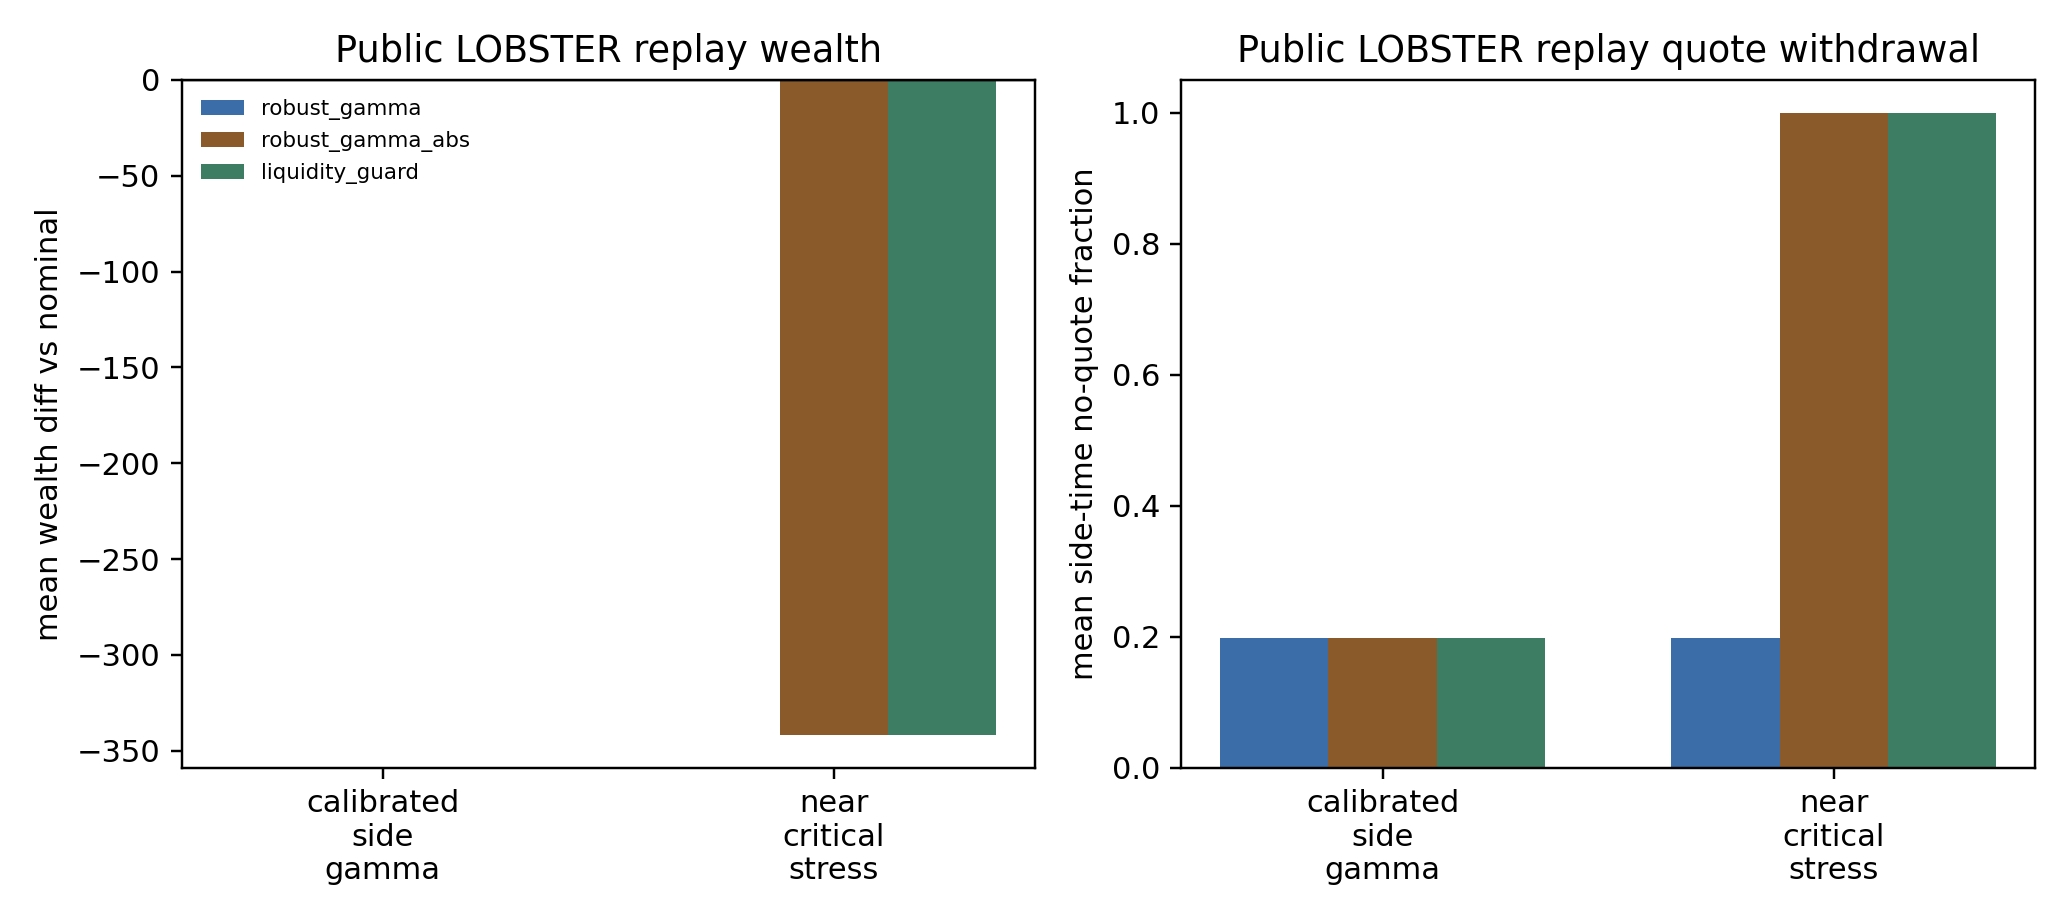
\includegraphics[width=.78\linewidth]{figures/lobster_top_of_book_replay.png}
\caption{Public LOBSTER top-of-book replay on actual message/order-book
streams. Calibrated policies coincide under the simple binary rule; in the
near-critical stress case, absolute-Gamma ambiguity withdraws quotes on the
same data paths.}
\end{figure}

\begin{figure}[!htbp]
\centering
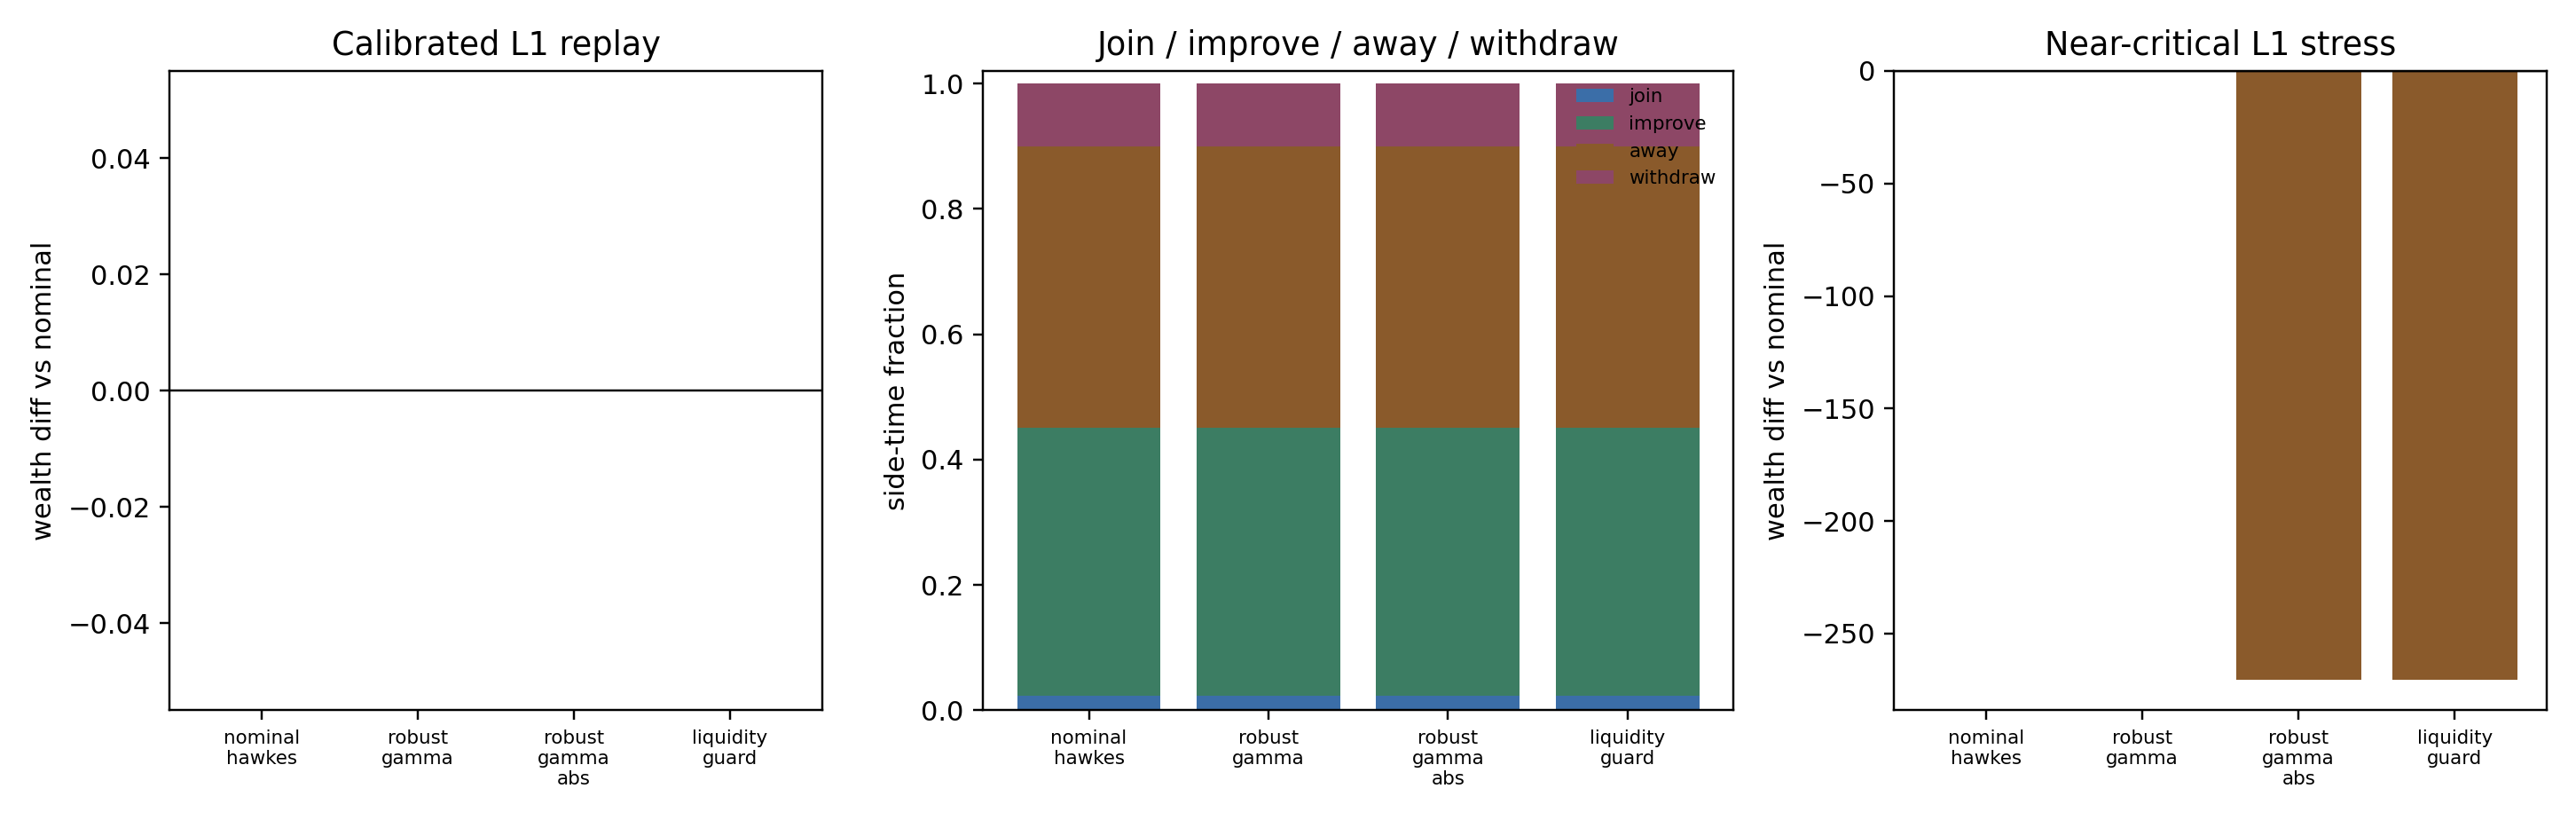
\includegraphics[width=.86\linewidth]{figures/lobster_l1_quote_replay.png}
\caption{Offset-aware L1 quote replay. Tick rounding still makes calibrated
policy wealth coincide, but the replay shows where quotes would be placed and
when near-critical absolute-Gamma ambiguity withdraws them.}
\end{figure}

\begin{figure}[!htbp]
\centering
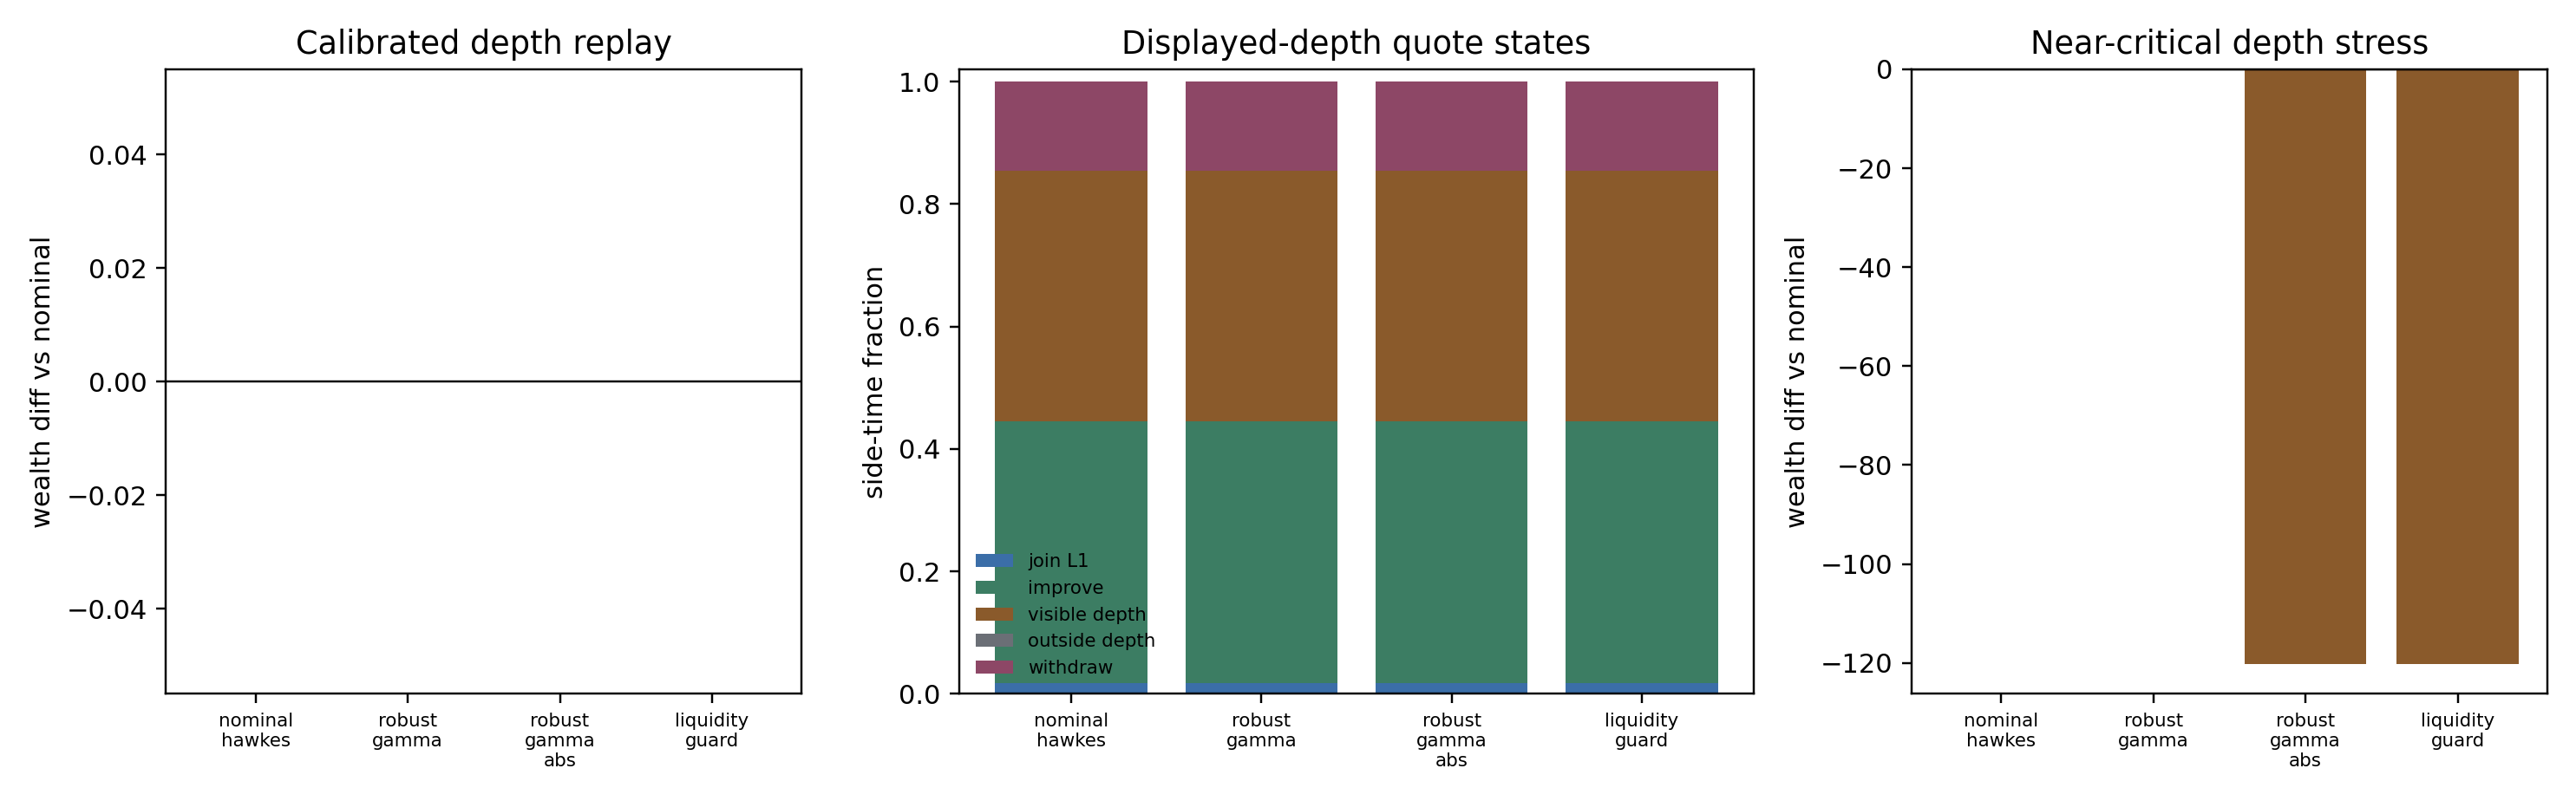
\includegraphics[width=.88\linewidth]{figures/lobster_depth_quote_replay.png}
\caption{Displayed-depth level-10 LOBSTER quote replay. Away-from-L1 quotes
can fill only when they rest inside the visible book and observed executions or
depth changes deplete displayed queue ahead.}
\end{figure}

\begin{figure}[!htbp]
\centering
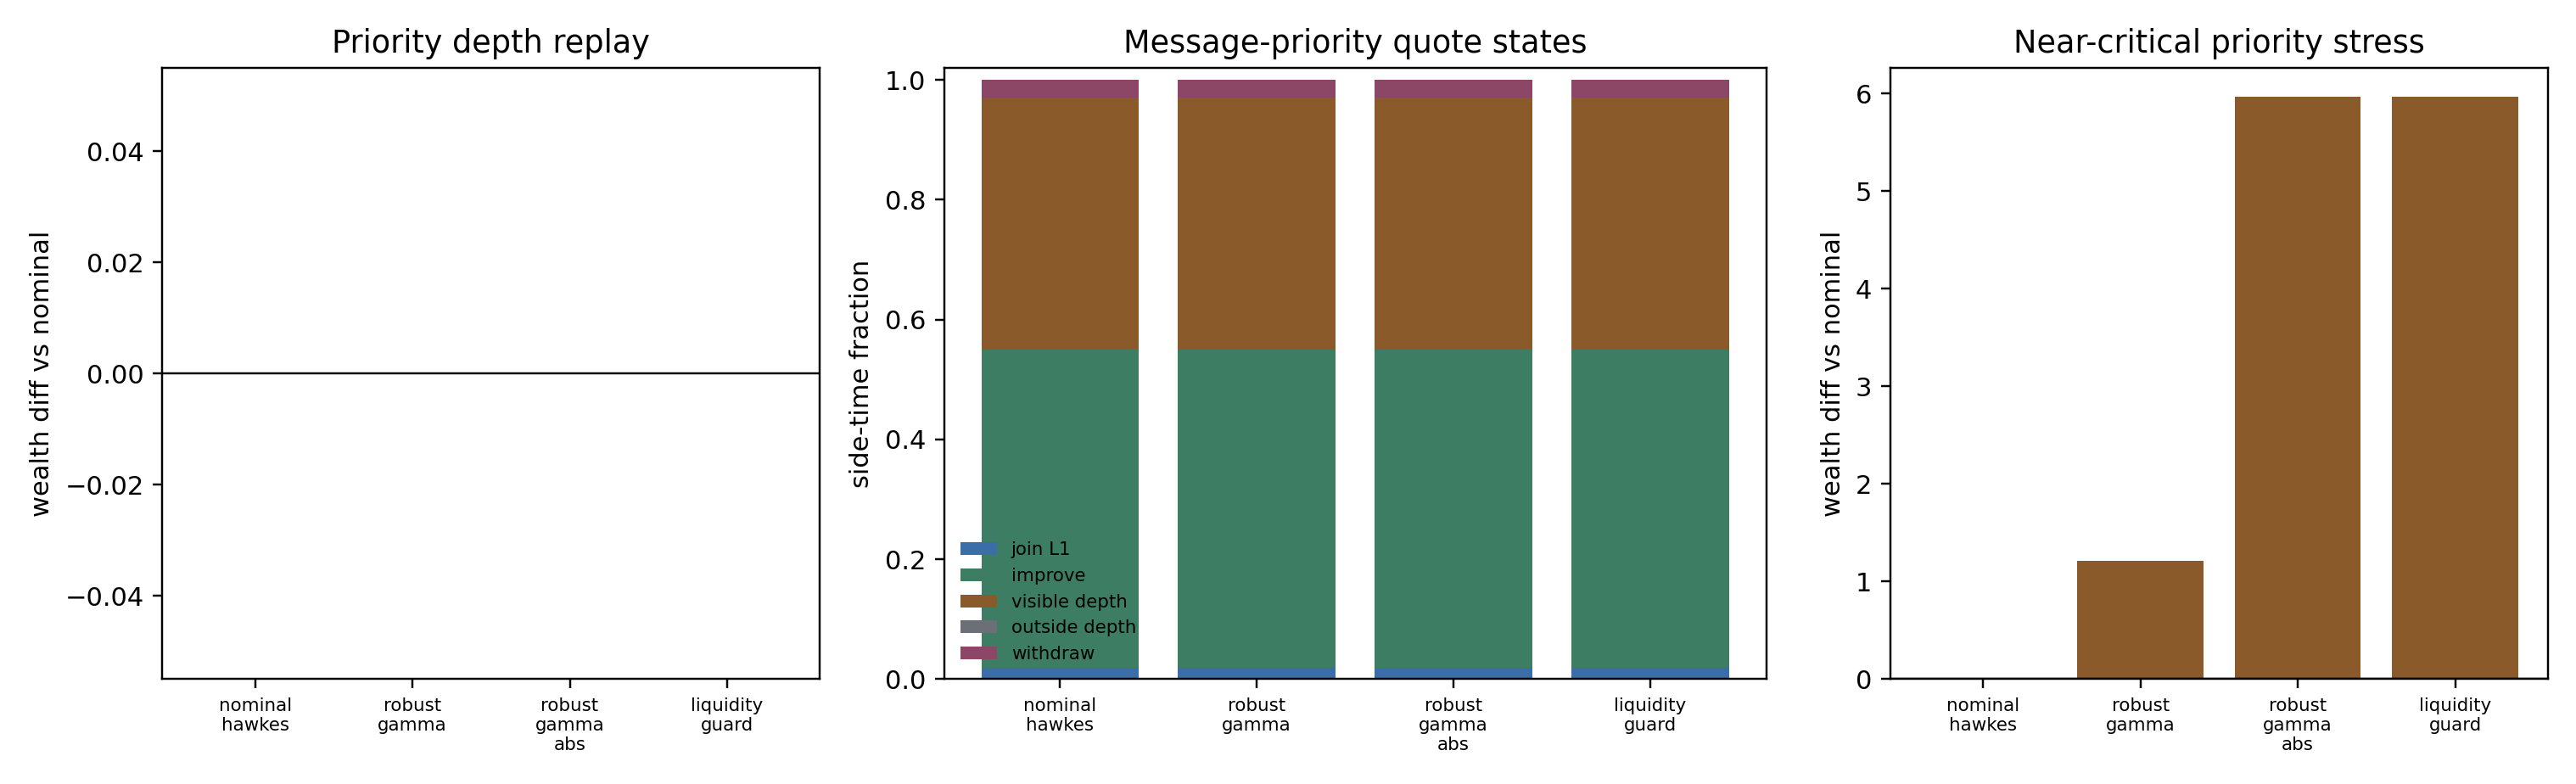
\includegraphics[width=.88\linewidth]{figures/lobster_priority_depth_quote_replay.png}
\caption{Residual-volume priority-aware level-10 LOBSTER quote replay.
Same-price orders arriving after the synthetic quote are kept behind it; queued
fills require residual execution volume after displayed queue-ahead depletion.}
\end{figure}

\begin{figure}[!htbp]
\centering
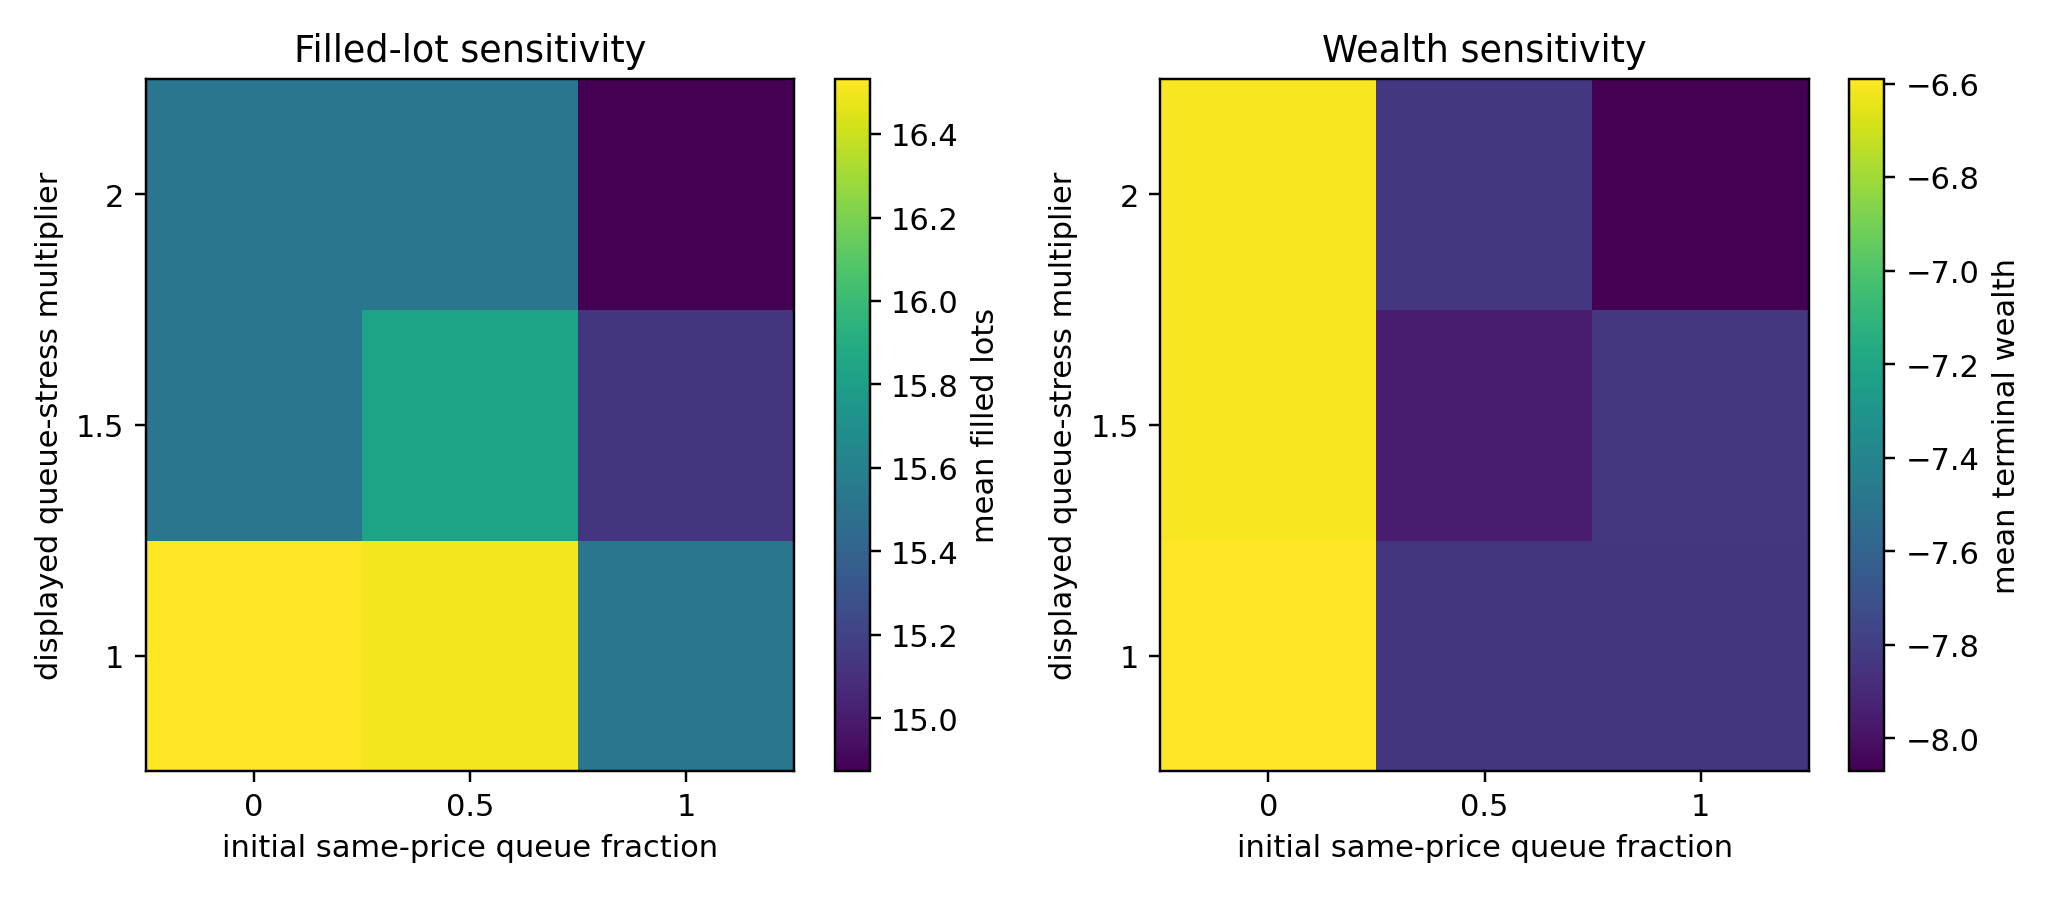
\includegraphics[width=.84\linewidth]{figures/lobster_priority_depth_sensitivity.png}
\caption{Priority-assumption sensitivity for the nominal level-10 replay. The
grid varies same-price displayed priority and displayed queue stress; filled
lots remain rare, showing the public-data limit of same-price priority
identification.}
\end{figure}

\begin{figure}[!htbp]
\centering
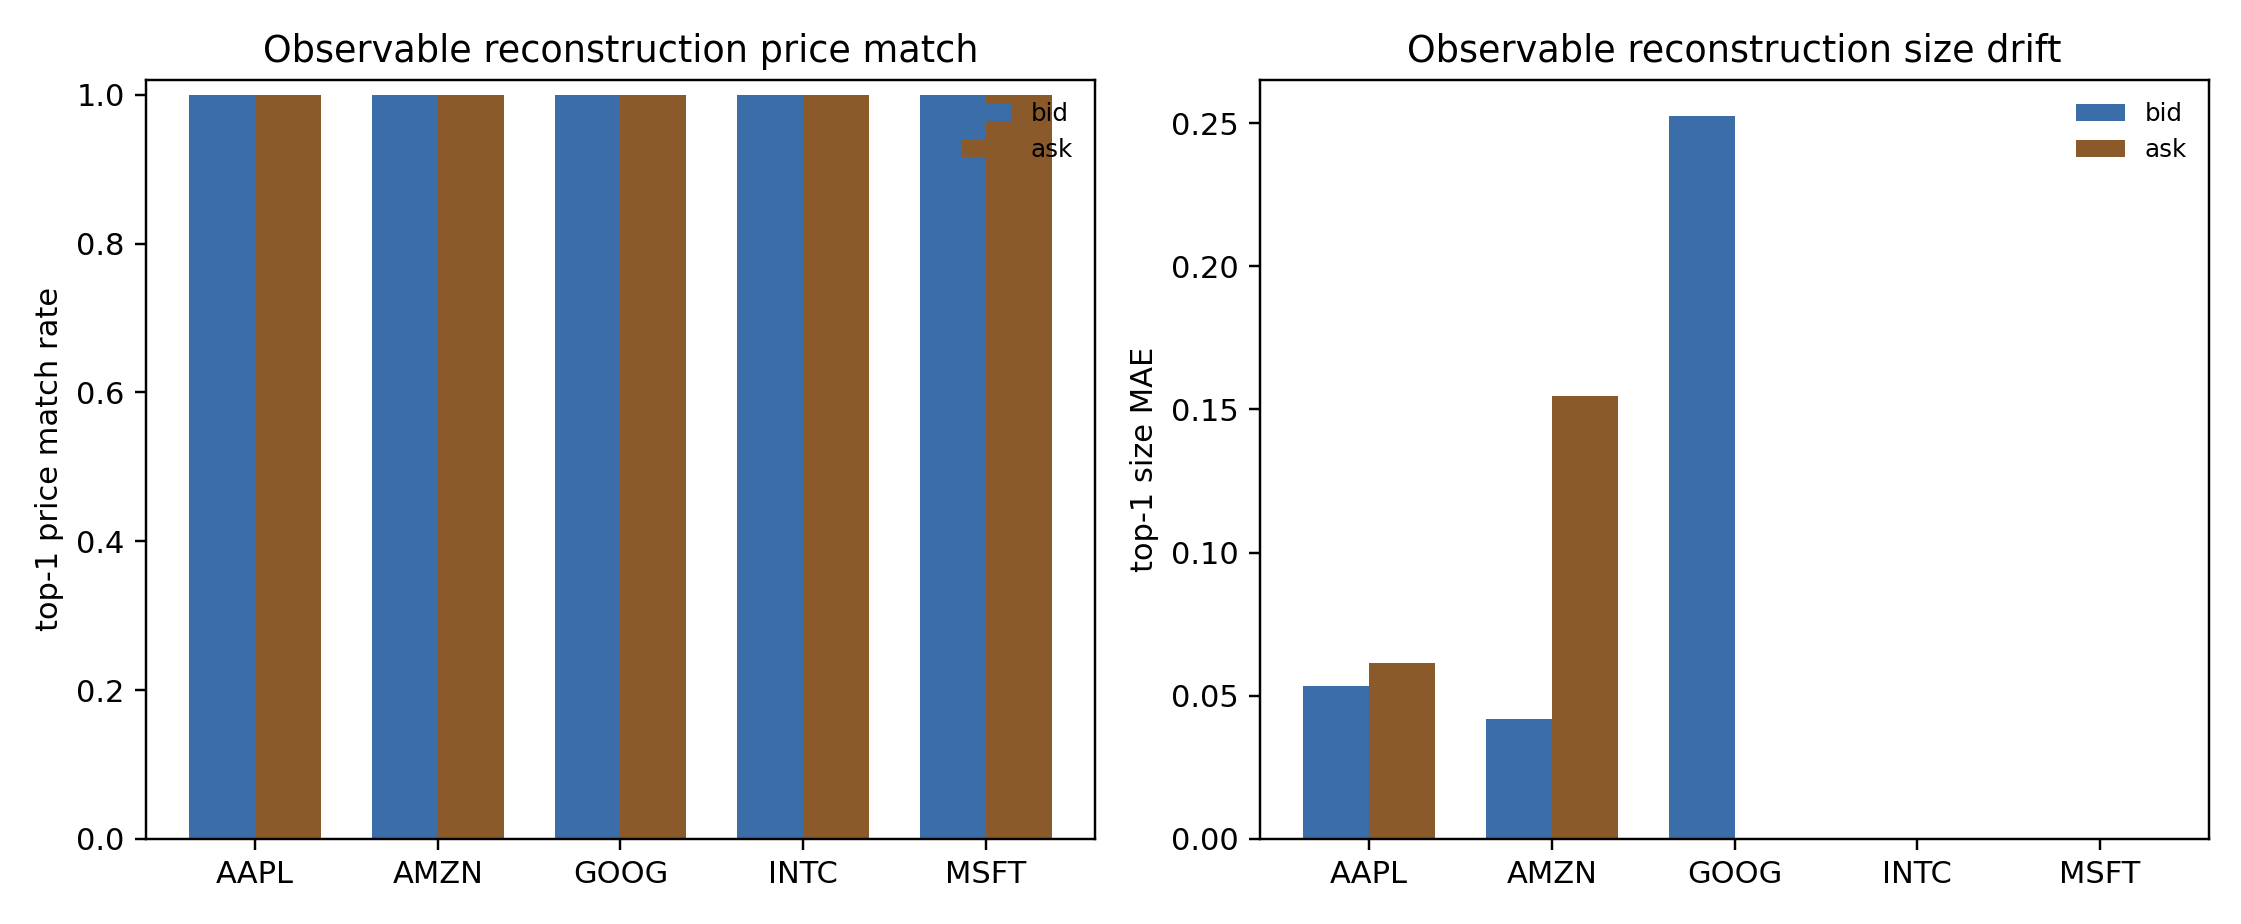
\includegraphics[width=.84\linewidth]{figures/lobster_orderbook_reconstruction.png}
\caption{Observable order-book reconstruction check. Re-anchored message-level
reconstruction matches top-of-book prices closely, while full-depth size drift
remains visible.}
\end{figure}

\FloatBarrier
\subsection{Simulator Validation}

The slow Ogata reference simulator makes the numerical issue visible:
coarse time discretization can create spurious critical amplification. At
$\rho=0.90$, the relative mean-count bias falls from $3.07$ at $\Delta t=0.08$
to $0.03$ at $\Delta t=0.01$. At $\rho=0.97$, even $\Delta t=0.005$ leaves
about $0.20$ relative bias in the current short-horizon setting.

\begin{figure}[!htbp]
\centering
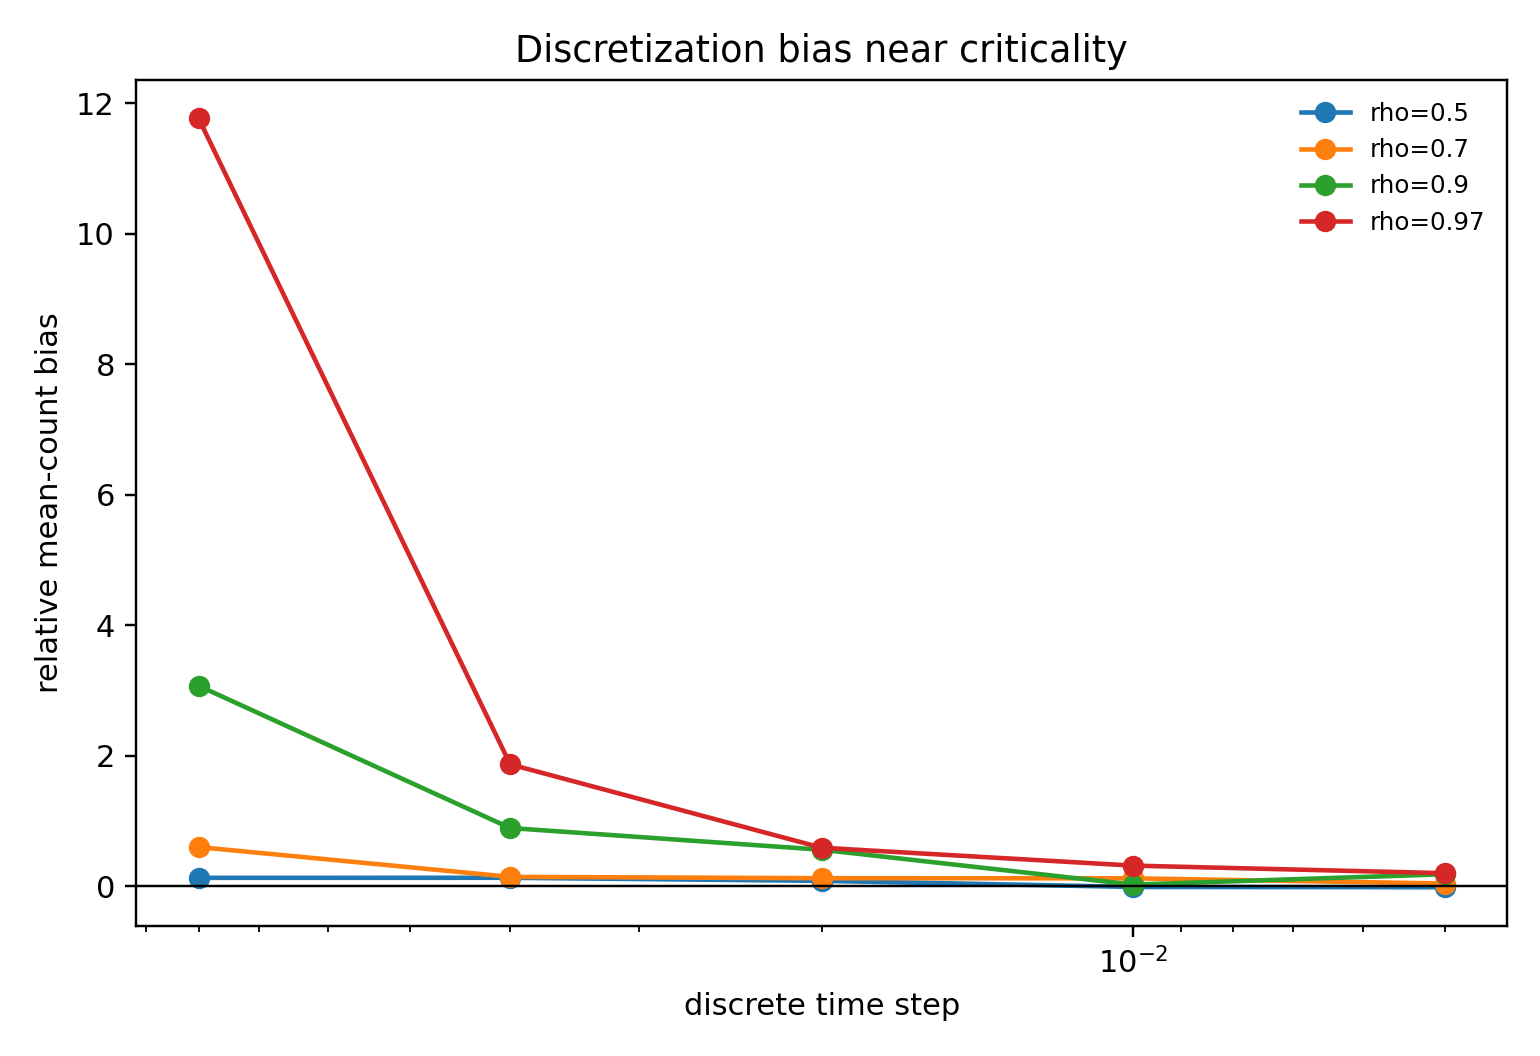
\includegraphics[width=.62\linewidth]{figures/discretization_bias.png}
\caption{Time-discretization bias grows sharply near criticality.}
\end{figure}

\FloatBarrier
\subsection{Calibration Noise}

A simple Fano-based criticality estimator points to the same practical concern:
near-critical calibration is fragile. For $\rho=0.97$, short horizons
under-estimate criticality, while longer horizons can over-shoot because rare
clusters dominate the count variance. This is why the empirical $\hat\rho$
estimates should be read with uncertainty, not as exact structural inputs.

\begin{figure}[!htbp]
\centering
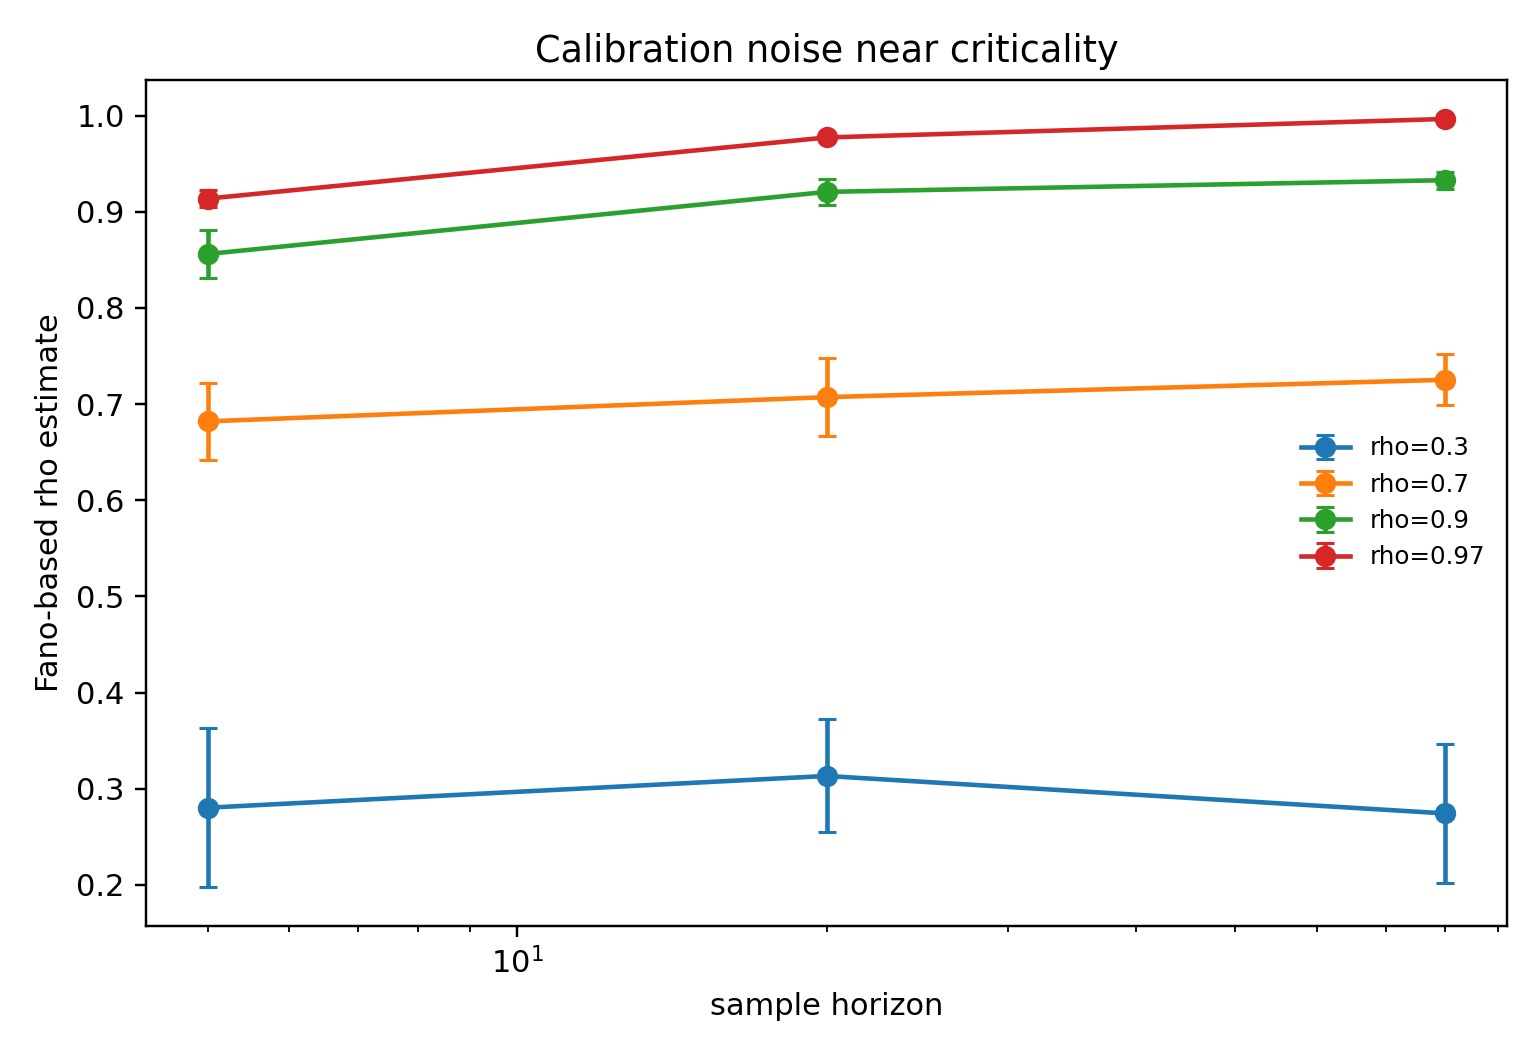
\includegraphics[width=.62\linewidth]{figures/calibration_noise.png}
\caption{Fano-based criticality estimates across horizons.}
\end{figure}

\FloatBarrier
\subsection{Robust Dynamic Programming}

The finite-scenario DP includes explicit bid-side and ask-side no-quote
actions. In the reported reduced run, the raw DP action grid contains 4,044
two-sided quote states, 618 bid-only states, 618 ask-only states, and no full
no-quote states. The first-step, zero-inventory rows remain two-sided through
the tested grid, which reaches $\hat\rho=0.92$. Averaged
over the DP grid, no-quote rates are $22.3\%$ under relative-slack ambiguity and
$24.5\%$ under absolute-Gamma ambiguity; full two-sided withdrawal rates are
zero for both. This is still a reduced Bellman approximation, not a
queue-calibrated quote-refusal simulator comparable one-for-one with
\cite{WangNoQuote2025}.

\begin{figure}[!htbp]
\centering
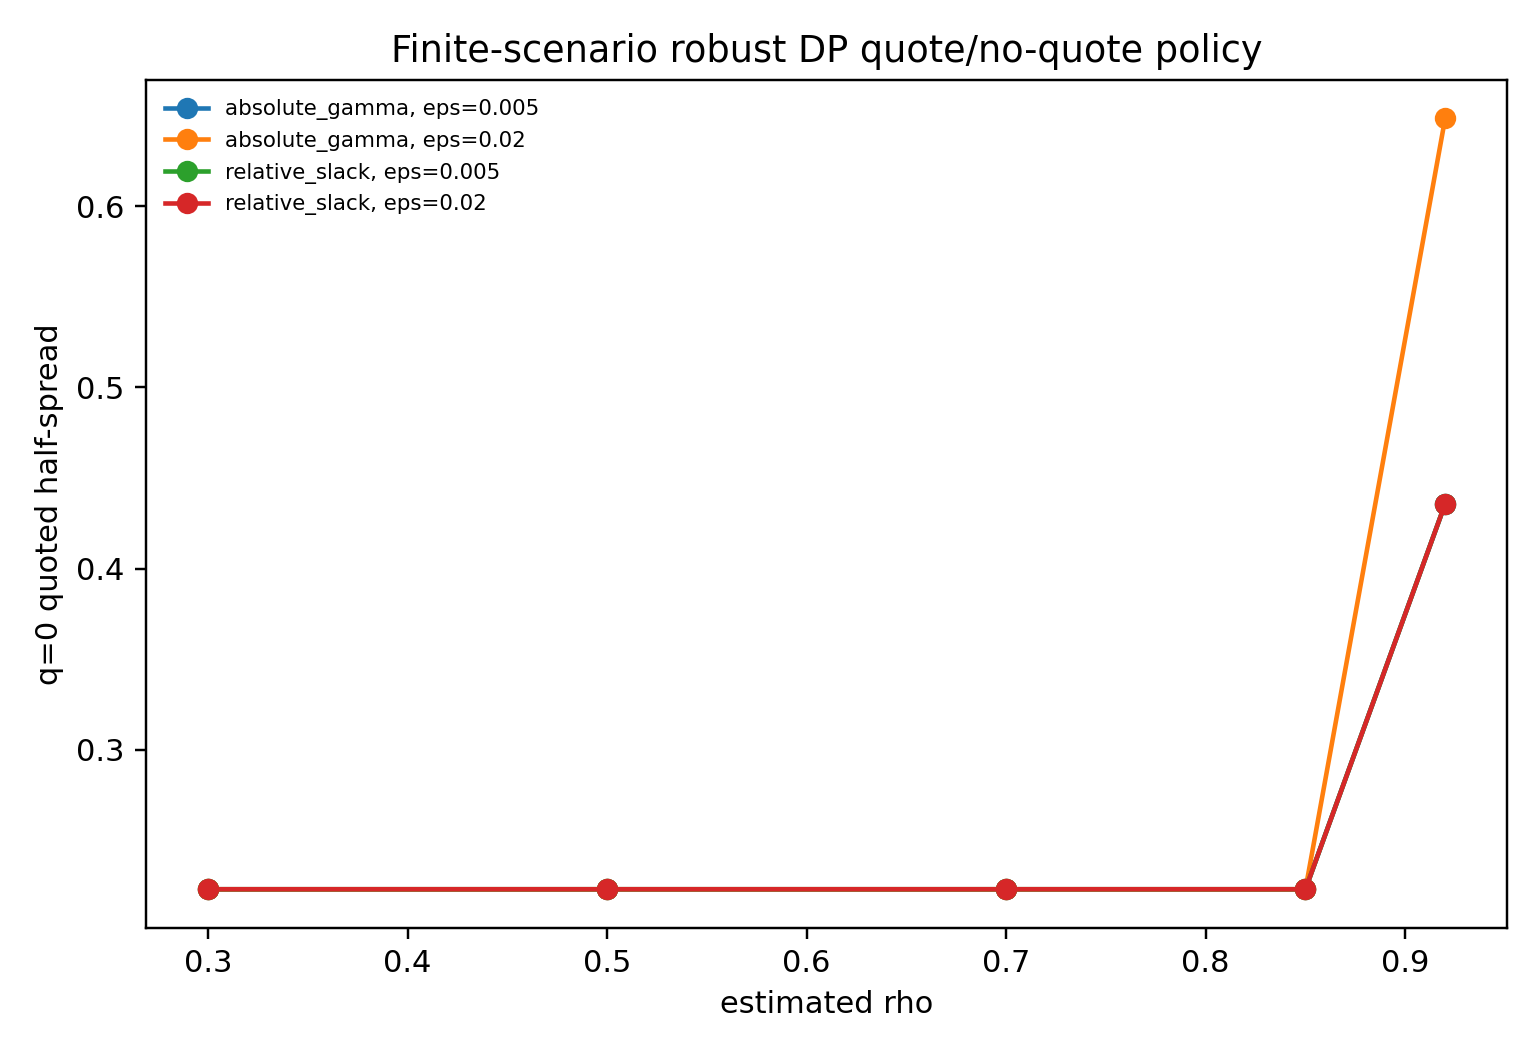
\includegraphics[width=.62\linewidth]{figures/robust_dp_quotes.png}
\caption{Reduced robust-DP half-spreads and no-quote switching as criticality
increases.}
\end{figure}

We also run a quote-map sensitivity diagnostic linking the local optimizer
theorem to the implemented policy map. For the smooth implemented half-spread,
nominal and relative-Gamma robust policies recover critical exponent $3.000$
for $d\delta/d\rho$, while absolute-Gamma robust policies approach exponent
$4.000$ in the uncapped interior region. Capped or no-quote points are marked
as nonsmooth active-set cases rather than treated as classical derivatives.

\begin{figure}[!htbp]
\centering
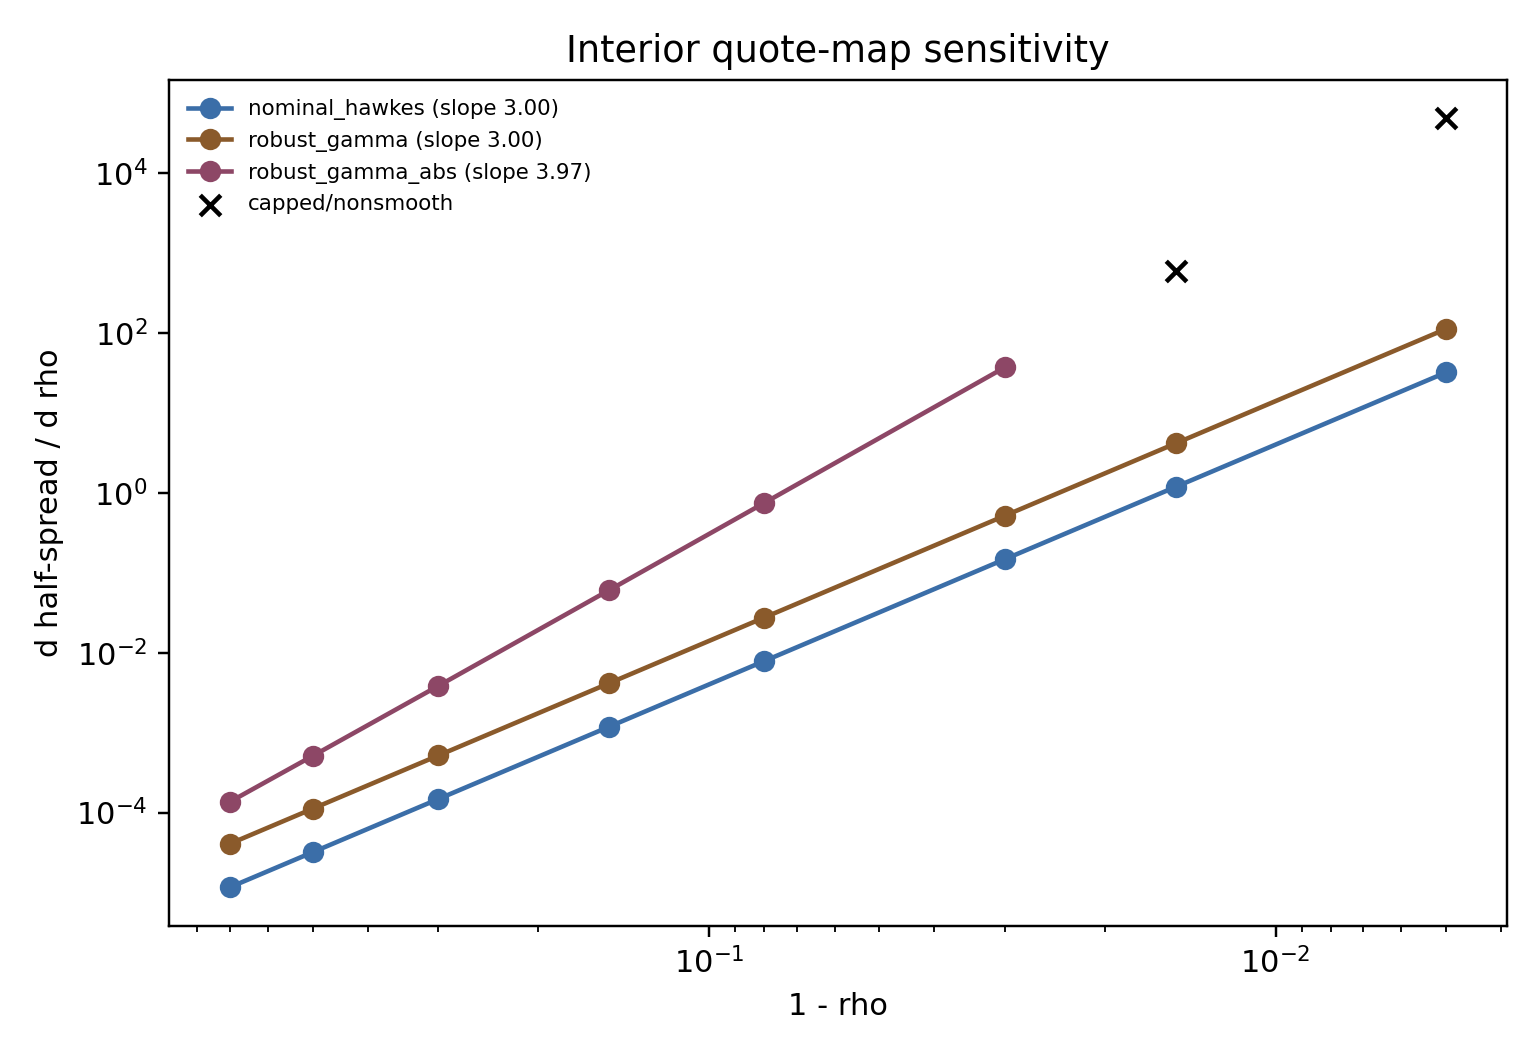
\includegraphics[width=.62\linewidth]{figures/quote_sensitivity_diagnostic.png}
\caption{Interior quote-map sensitivity. Smooth relative-Gamma policies have
third-order derivative blowup, while absolute-Gamma ambiguity adds one more
critical derivative factor until spread caps bind.}
\end{figure}

\FloatBarrier
\subsection{Public Data Panels}

The public datasets are not used to prove the structural ambiguity theorem,
because the true $\Gamma$ is unobserved. Instead, they document clustered order
flow and overdispersed liquidity states in the data used for the diagnostics.
Binance aggregate trades are fetched from the public archive at
\url{https://data.binance.vision/?prefix=data/spot/daily/aggTrades/}.

\begin{table}[!htbp]
\centering
\small
\begin{tabular}{@{}lrrrr@{}}
\toprule
Ticker & Rows & Events/sec & Event Fano & Mean spread \\
\midrule
AAPL & 118497 & 5.064 & 19.460 & 0.155 \\
AMZN & 57515 & 2.458 & 13.329 & 0.136 \\
GOOG & 49482 & 2.115 & 17.185 & 0.311 \\
INTC & 404986 & 17.307 & 220.650 & 0.013 \\
MSFT & 411409 & 17.582 & 196.485 & 0.013 \\
\bottomrule
\end{tabular}
\caption{Public LOBSTER sample sanity panel.}
\end{table}

\begin{table}[!htbp]
\centering
\small
\begin{tabular}{@{}lrrrr@{}}
\toprule
Symbol & Agg. trades & Agg. trades/sec & Event Fano & ACF1 \\
\midrule
BTCUSDT & 1364603 & 15.794 & 200.274 & 0.342 \\
ETHUSDT & 597417 & 6.915 & 29.730 & 0.241 \\
SOLUSDT & 218278 & 2.526 & 12.240 & 0.201 \\
\bottomrule
\end{tabular}
\caption{Public Binance aggregate-trade event panel for 2024-01-15.}
\end{table}

\begin{table}[!htbp]
\centering
\small
\begin{tabular}{@{}lrrrr@{}}
\toprule
Symbol & Rows & Rel. spread bps & Return std & Depth Fano \\
\midrule
BTC & 10081 & 0.163 & 0.000687 & 33.989 \\
ETH & 10081 & 0.591 & 0.000910 & 513.703 \\
SOL & 10080 & 0.911 & 0.001110 & 1697.605 \\
\bottomrule
\end{tabular}
\caption{Public crypto L2 depth sanity panel.}
\end{table}

\begin{figure}[!htbp]
\centering
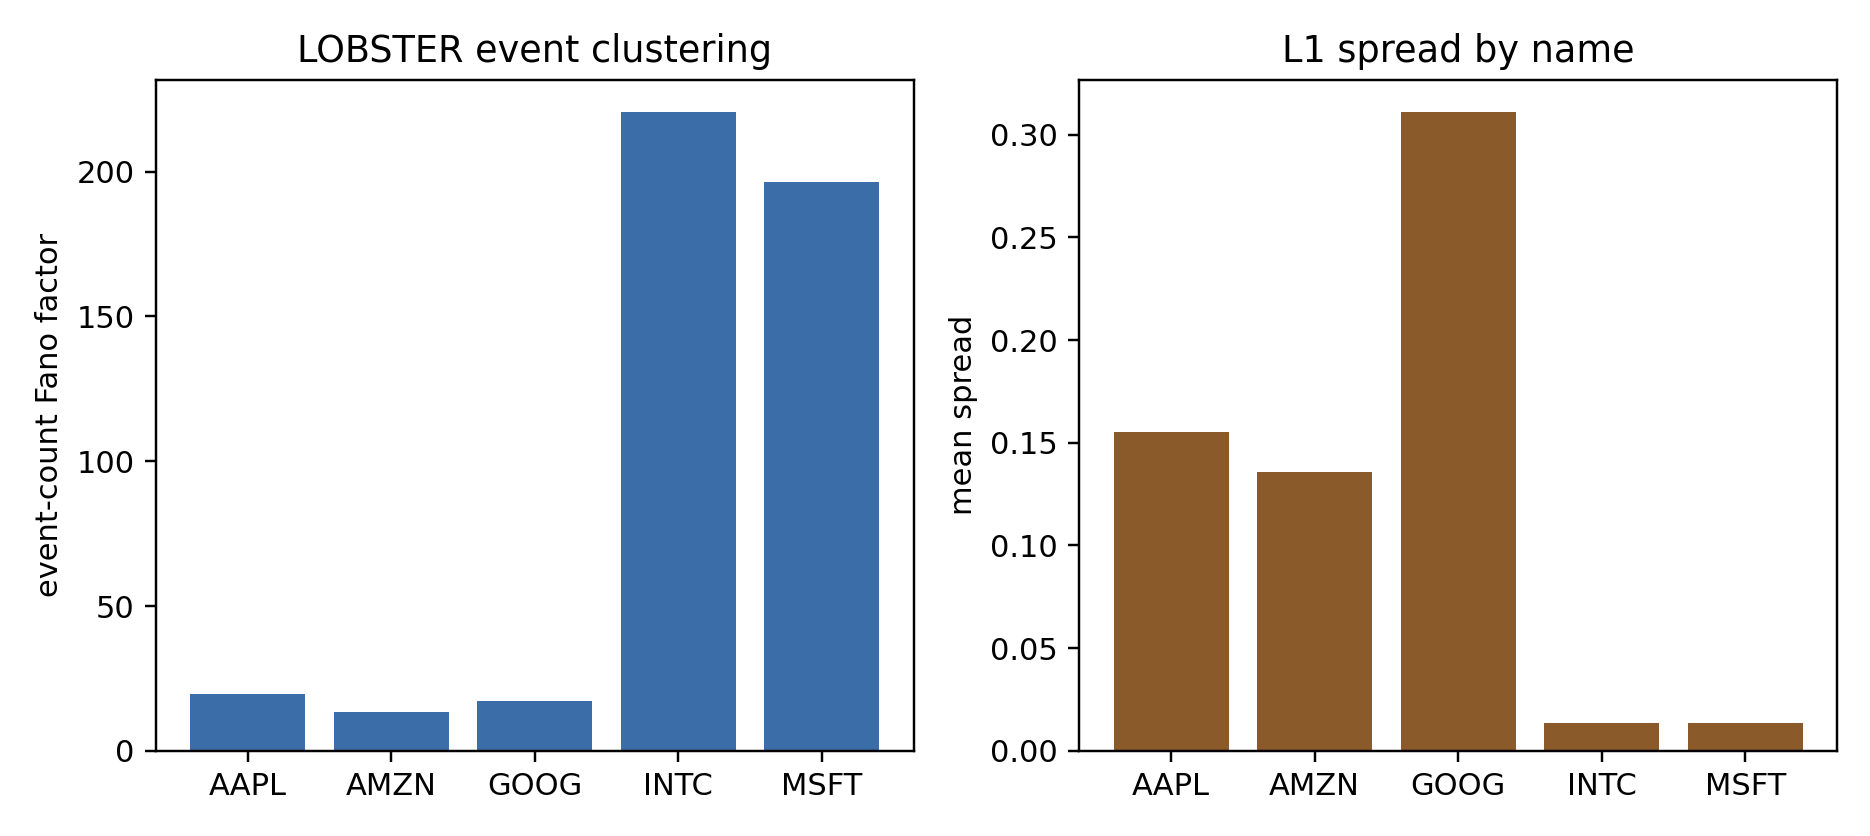
\includegraphics[width=.48\linewidth]{figures/lobster_panel_sanity.png}
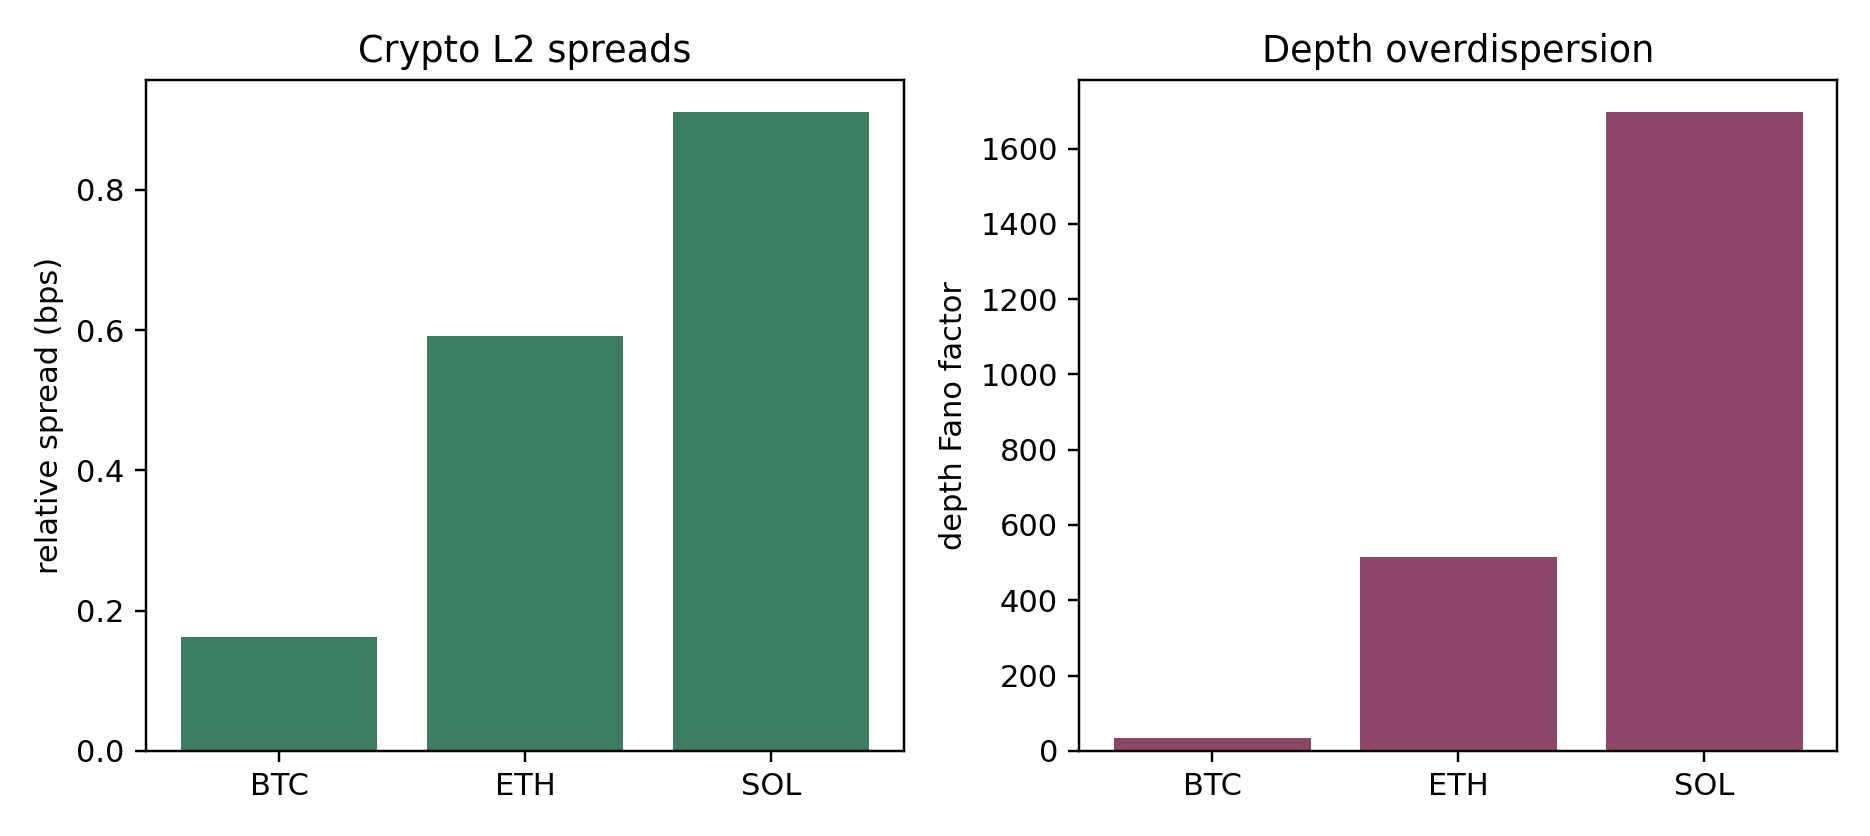
\includegraphics[width=.48\linewidth]{figures/crypto_l2_sanity.png}
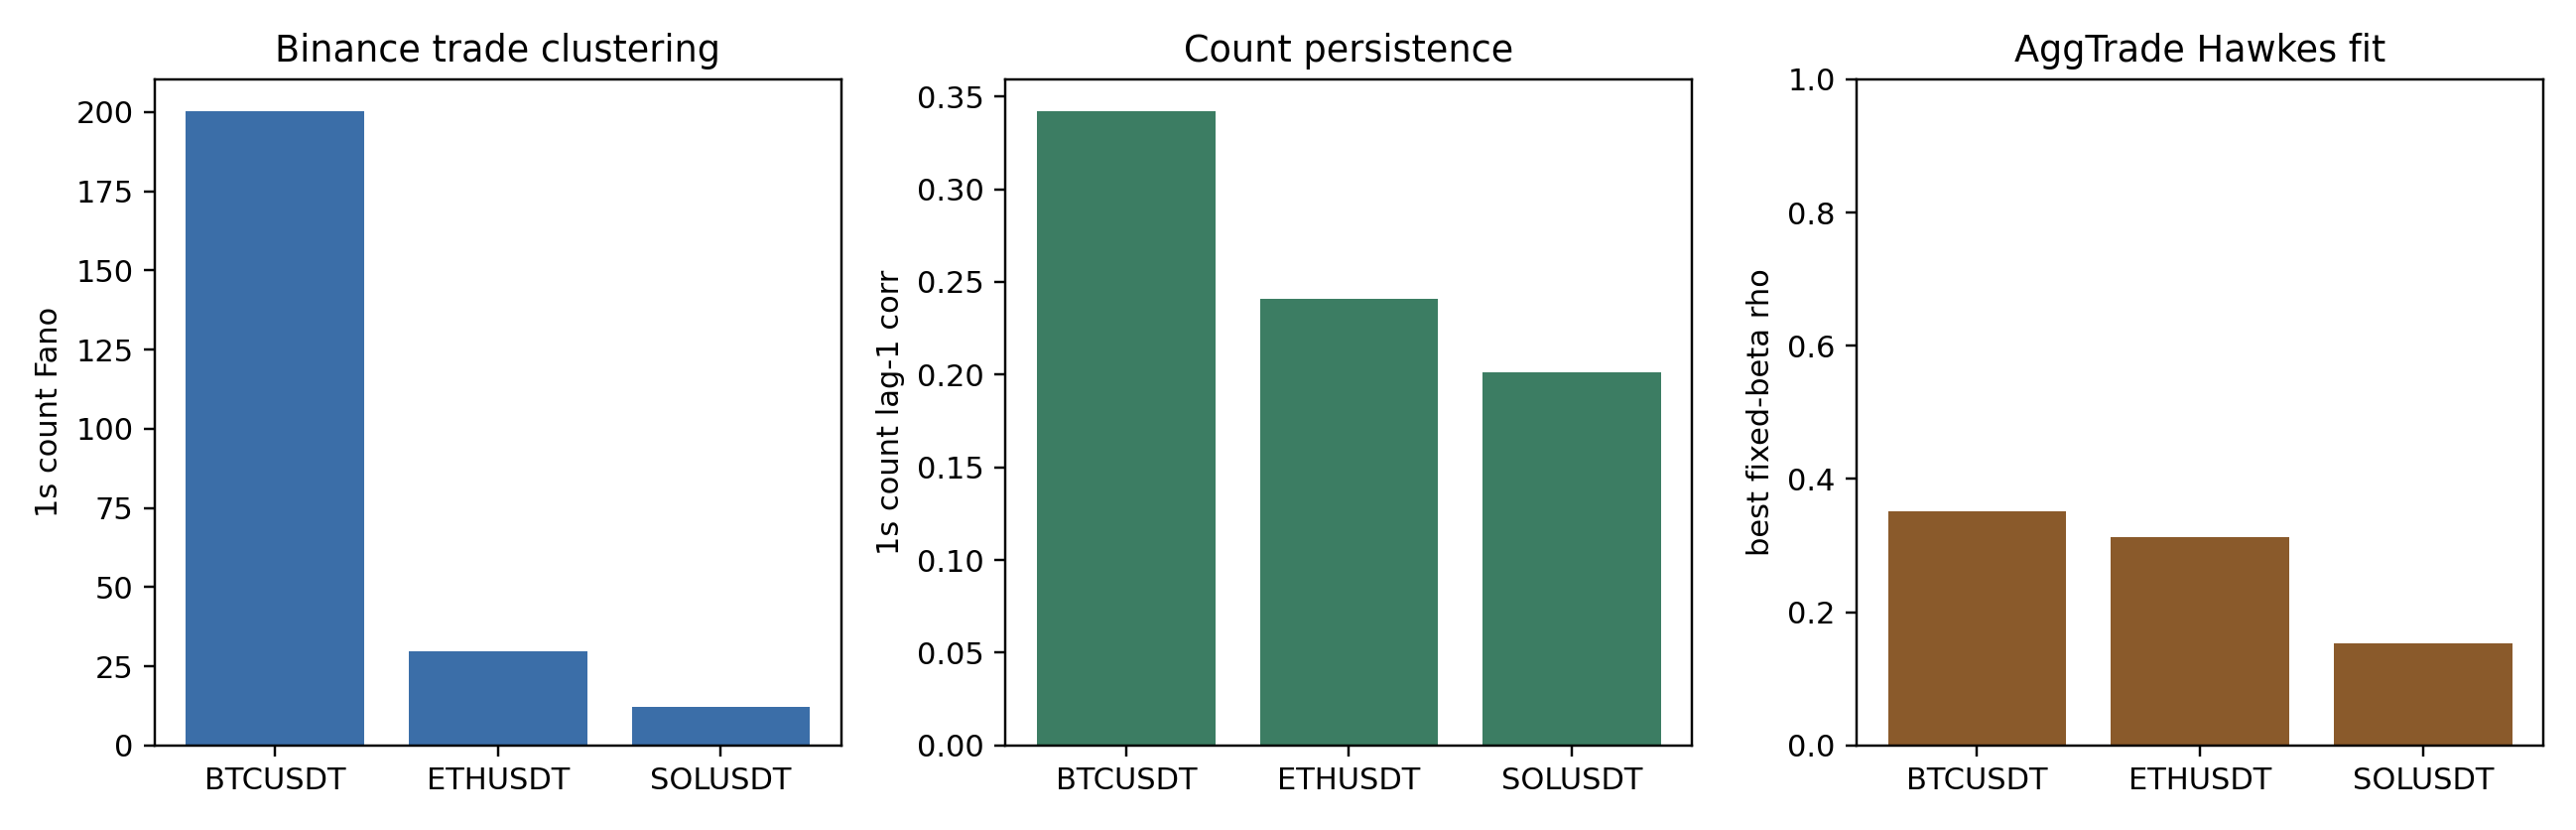
\includegraphics[width=.78\linewidth]{figures/binance_aggtrades_hawkes.png}
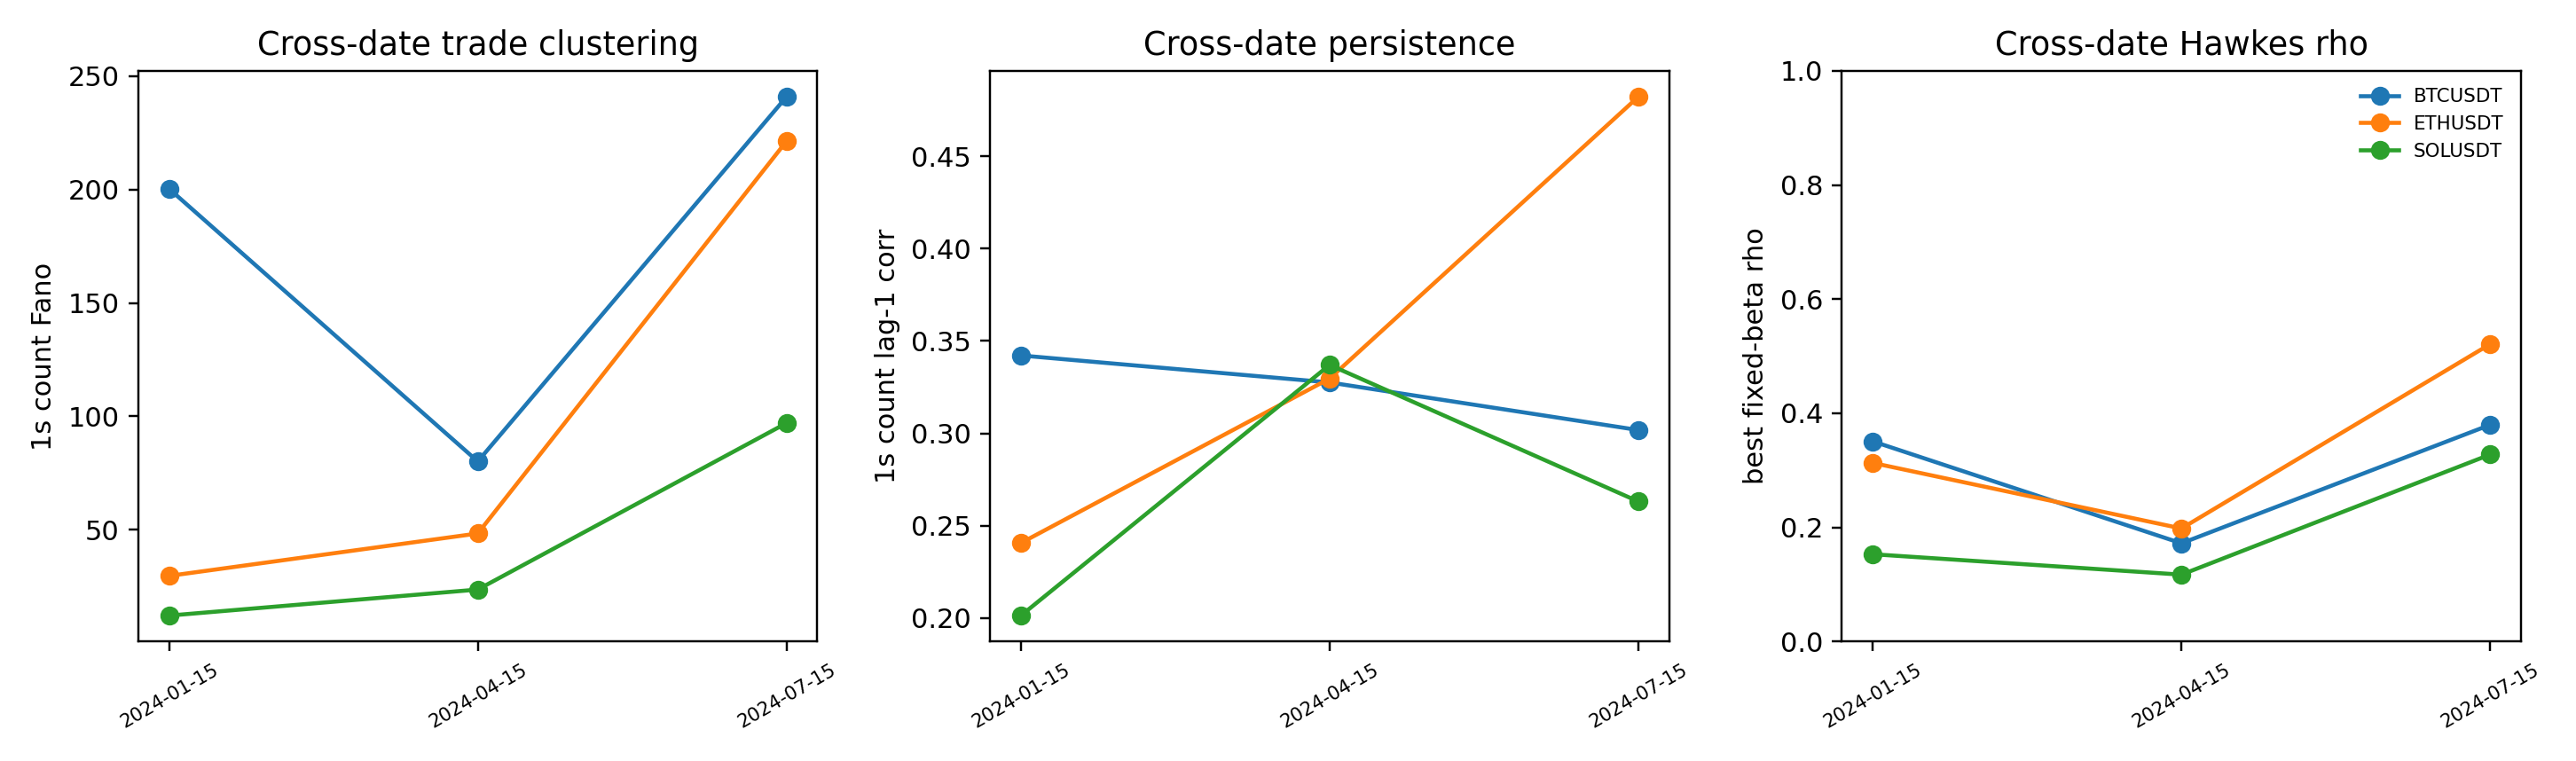
\includegraphics[width=.82\linewidth]{figures/binance_aggtrades_cross_date_hawkes.png}
\caption{Public-data sanity figures: LOBSTER event clustering and spreads,
crypto L2 spreads and depth overdispersion, Binance aggregate-trade clustering,
fixed-beta Hawkes diagnostics, and cross-date robustness.}
\end{figure}

\FloatBarrier
\subsection{Corrected Hawkes Calibration Diagnostics}

As a check before interpreting real-data Hawkes fits, we validate the corrected
single-exponential MLE on Ogata-simulated paths with known parameters. The
validation recovers moderate and near-critical branching ratios without
beta-bound failures.

\begin{table}[!htbp]
\centering
\small
\begin{tabular}{@{}rrrrr@{}}
\toprule
$\rho$ true & $\beta$ true & $\rho$ MAE & $\beta$ MAPE & Beta cap rate \\
\midrule
0.30 & 2.0 & 0.043 & 0.201 & 0.000 \\
0.70 & 4.0 & 0.019 & 0.026 & 0.000 \\
0.90 & 8.0 & 0.016 & 0.039 & 0.000 \\
\bottomrule
\end{tabular}
\caption{Synthetic Ogata validation for the corrected Hawkes MLE.}
\end{table}

We also validate the fixed-beta marked multivariate estimator on
three-type Ogata Hawkes paths with known branching matrices. For target
spectral radii $0.35$ and $0.65$ at $\beta=3$, the marked estimator has
spectral-radius MAE $0.025$ and $0.023$, relative Frobenius branching-matrix
error $0.234$ and $0.133$, and a success rate of $1.000$. This check is important
because the public-data marked calibrations below are only meaningful if the
estimator can recover a known multitype $\Gamma$ under controlled simulation.

\begin{table}[!htbp]
\centering
\small
\begin{tabular}{@{}rrrrr@{}}
\toprule
$\rho$ true & Mean events & $\rho$ MAE & $\|\hat\Gamma-\Gamma\|_F/\|\Gamma\|_F$ & Success \\
\midrule
0.35 & 1209.8 & 0.025 & 0.234 & 1.000 \\
0.65 & 2171.2 & 0.023 & 0.133 & 1.000 \\
\bottomrule
\end{tabular}
\caption{Synthetic Ogata validation for the fixed-beta marked multivariate
Hawkes estimator.}
\end{table}

\begin{figure}[!htbp]
\centering
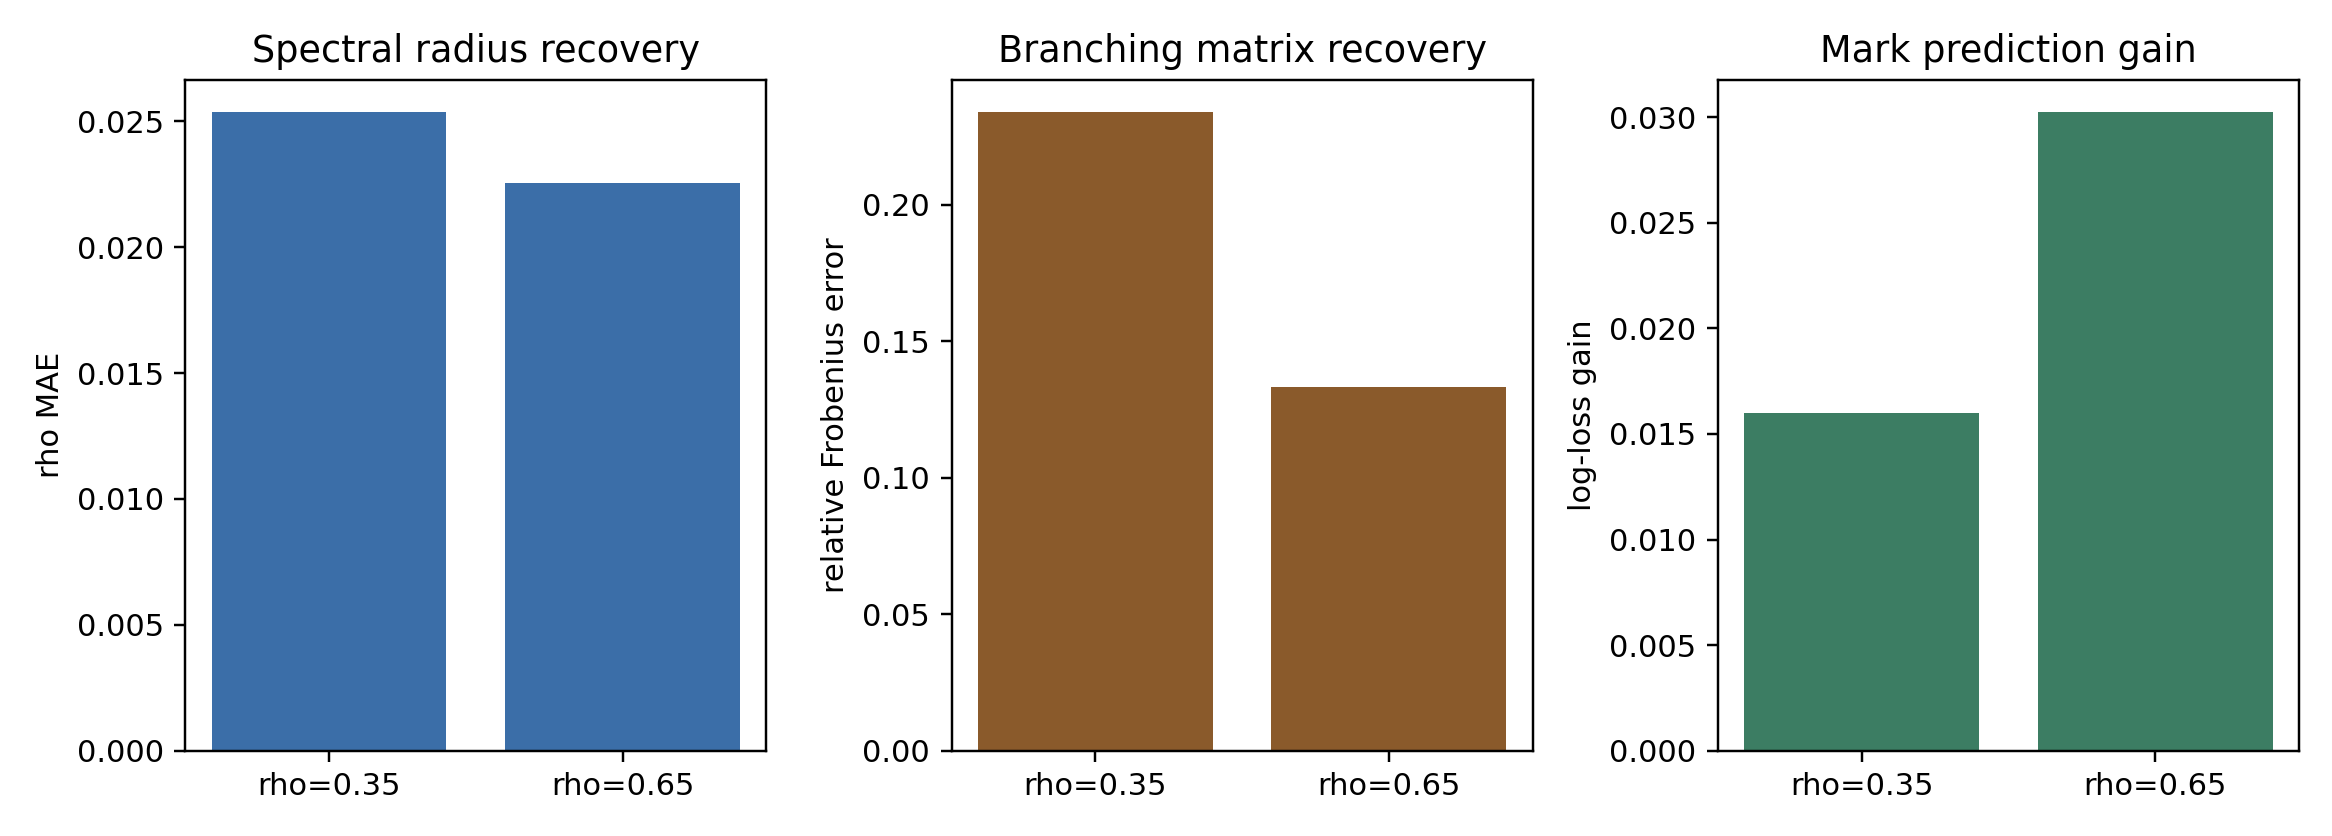
\includegraphics[width=.76\linewidth]{figures/lobster_marked_hawkes_estimator_validation.png}
\caption{Marked multivariate Ogata validation: spectral-radius recovery,
branching-matrix recovery, and conditional mark-prediction gain.}
\end{figure}

The Binance aggregate-trade panel provides a separate public check on crypto
event clustering. On 2024-01-15, BTCUSDT, ETHUSDT, and SOLUSDT have 218k to
1.36m
aggregate trades, one-second event-count Fano factors from $12.24$ to
$200.27$, and lag-one count autocorrelations from $0.201$ to $0.342$. Fixed
beta Hawkes fits over all aggregate trades, buy-aggressor trades, and
sell-aggressor trades select $\beta=100$ in the current grid. All-trade
branching ratios are $0.351$ for BTCUSDT, $0.313$ for ETHUSDT, and $0.153$ for
SOLUSDT; sell-aggressor branching is higher for BTCUSDT and ETHUSDT, at
$0.493$ and $0.463$. This is useful cross-asset evidence of clustered event
flow, but aggregate trades do not include order placement, cancellation, or
queue state, so the panel should not be read as an execution benchmark.

To avoid relying on one crypto day, we repeat the Binance check on
2024-01-15, 2024-04-15, and 2024-07-15. Across all-event fixed-beta fits,
branching-ratio ranges are $0.172$--$0.380$ for BTCUSDT, $0.198$--$0.521$ for
ETHUSDT, and $0.117$--$0.328$ for SOLUSDT. The median all-event branching
ratios remain $0.351$, $0.313$, and $0.153$, respectively.

On raw LOBSTER message arrivals, the all-message single-exponential fit remains
a misspecification diagnostic rather than a structural calibration target. The
corrected all-message panel still places $\beta$ at the upper
bound for every ticker under the 100k-event cap, with fitted branching ratios
between $0.64$ and $0.76$. Event-type splits and fixed-beta profiles show that
branching estimates are sensitive to the assumed decay scale; timestamp
aggregation sharply reduces the fitted decay, with median $\beta$ falling from
$148.4$ on raw events to $23.4$ at 1ms aggregation and $1.46$ at 10ms
aggregation. A fixed-beta two-scale diagnostic adds a multiscale check
but does not remove the misspecification warning: among the tested pairs, every
ticker/event-group selects $(\beta_{\rm slow},\beta_{\rm fast})=(1,100)$, and
median fast-excitation shares are $0.764$ for all messages, $0.723$ for limits,
$0.660$ for cancel/delete events, and $0.871$ for executions. Execution events
remain the hardest to fit, with median residual KS statistic about $0.415$.
This supports the methodological point that raw unmarked message flows mix
multiple clocks and packet-level bursts, so, in this setting, robust
market-making experiments should either use marked or multiscale calibration
diagnostics, or report residual diagnostics
\cite{BacryMuzy2015,Ogata1988}.

The package therefore also includes a grouped marked multivariate Hawkes fit on
limit, cancel/delete, and execution event groups. With fixed exponential decay,
AIC selects $\beta=100$ for all five public LOBSTER tickers. The estimated
branching matrices are stable, with spectral radii from $0.367$ to $0.622$,
and the conditional mark log-loss improves over unconditional event-frequency
prediction by $0.005$ to $0.114$ nats per event. The median branching matrix
has the strongest source column from execution events, with median total
outgoing branching about $0.923$, and the largest median target row into limit
intensity, about $0.897$. Residual KS statistics still range from $0.050$ to
$0.217$, so the fit should be read as a reproducible marked calibration
diagnostic, not as a production-grade structural $\Gamma$ estimate.

Finally, to align the empirical object with the bid/ask control model, we fit a
six-mark side-aware Hawkes model using LOBSTER direction labels: limit,
cancel/delete, and execution events on buy and sell sides. AIC again selects
$\beta=100$ for all five tickers. The full six-mark branching matrices remain
stable, with spectral radii from $0.369$ to $0.624$, while conditional
six-mark log-loss improves over unconditional mark frequencies by $0.101$ to
$0.292$ nats per event. Median side-aggregated branching is strongest within
side, about $1.354$ from buy to buy and $1.403$ from sell to sell, with smaller
cross-side totals of about $0.492$ from buy to sell and $0.414$ from sell to
buy. The aggregate row sums can exceed one because they sum many target/source
entries; stability is assessed by the spectral radius of the full six-mark
matrix.

We then condition the six-mark time-rescaling residuals on observable L1 state
variables: event group, side, within-ticker size bucket, spread bucket,
top-depth bucket, and order-book imbalance bucket. This is a misspecification
check rather than another fitted model. Across the five
public LOBSTER samples, wide-spread states have median residual mean $0.886$
and median KS statistic $0.220$, while tight-spread states have median residual
mean $1.110$ and median KS statistic $0.092$. Large-size events have residual
mean $0.828$ versus $1.018$ for small events. Execution marks show the largest
conditional mark-prediction gain, with median log-loss improvement $0.384$
nats per event. The result sharpens the empirical conclusion: side-aware
excitation is informative, but the residuals still depend materially on size
and book state.

\begin{figure}[!htbp]
\centering
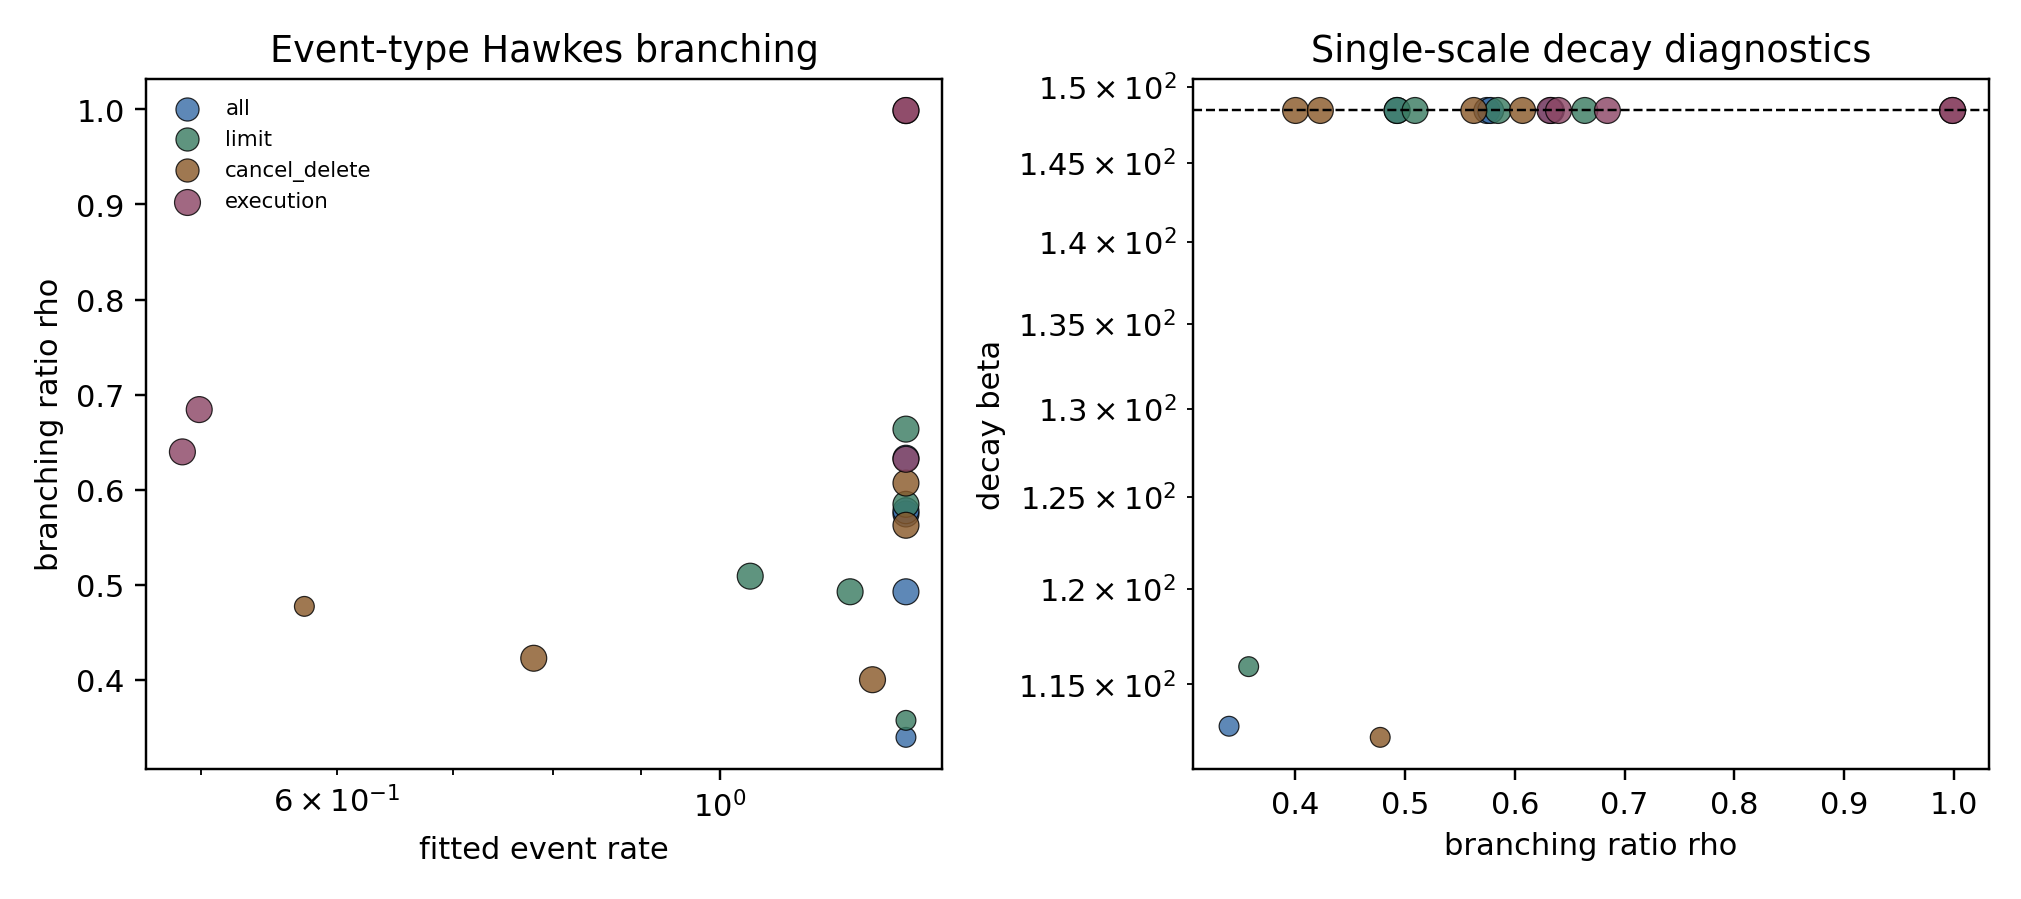
\includegraphics[width=.49\linewidth]{figures/lobster_hawkes_event_type_rho_beta.png}
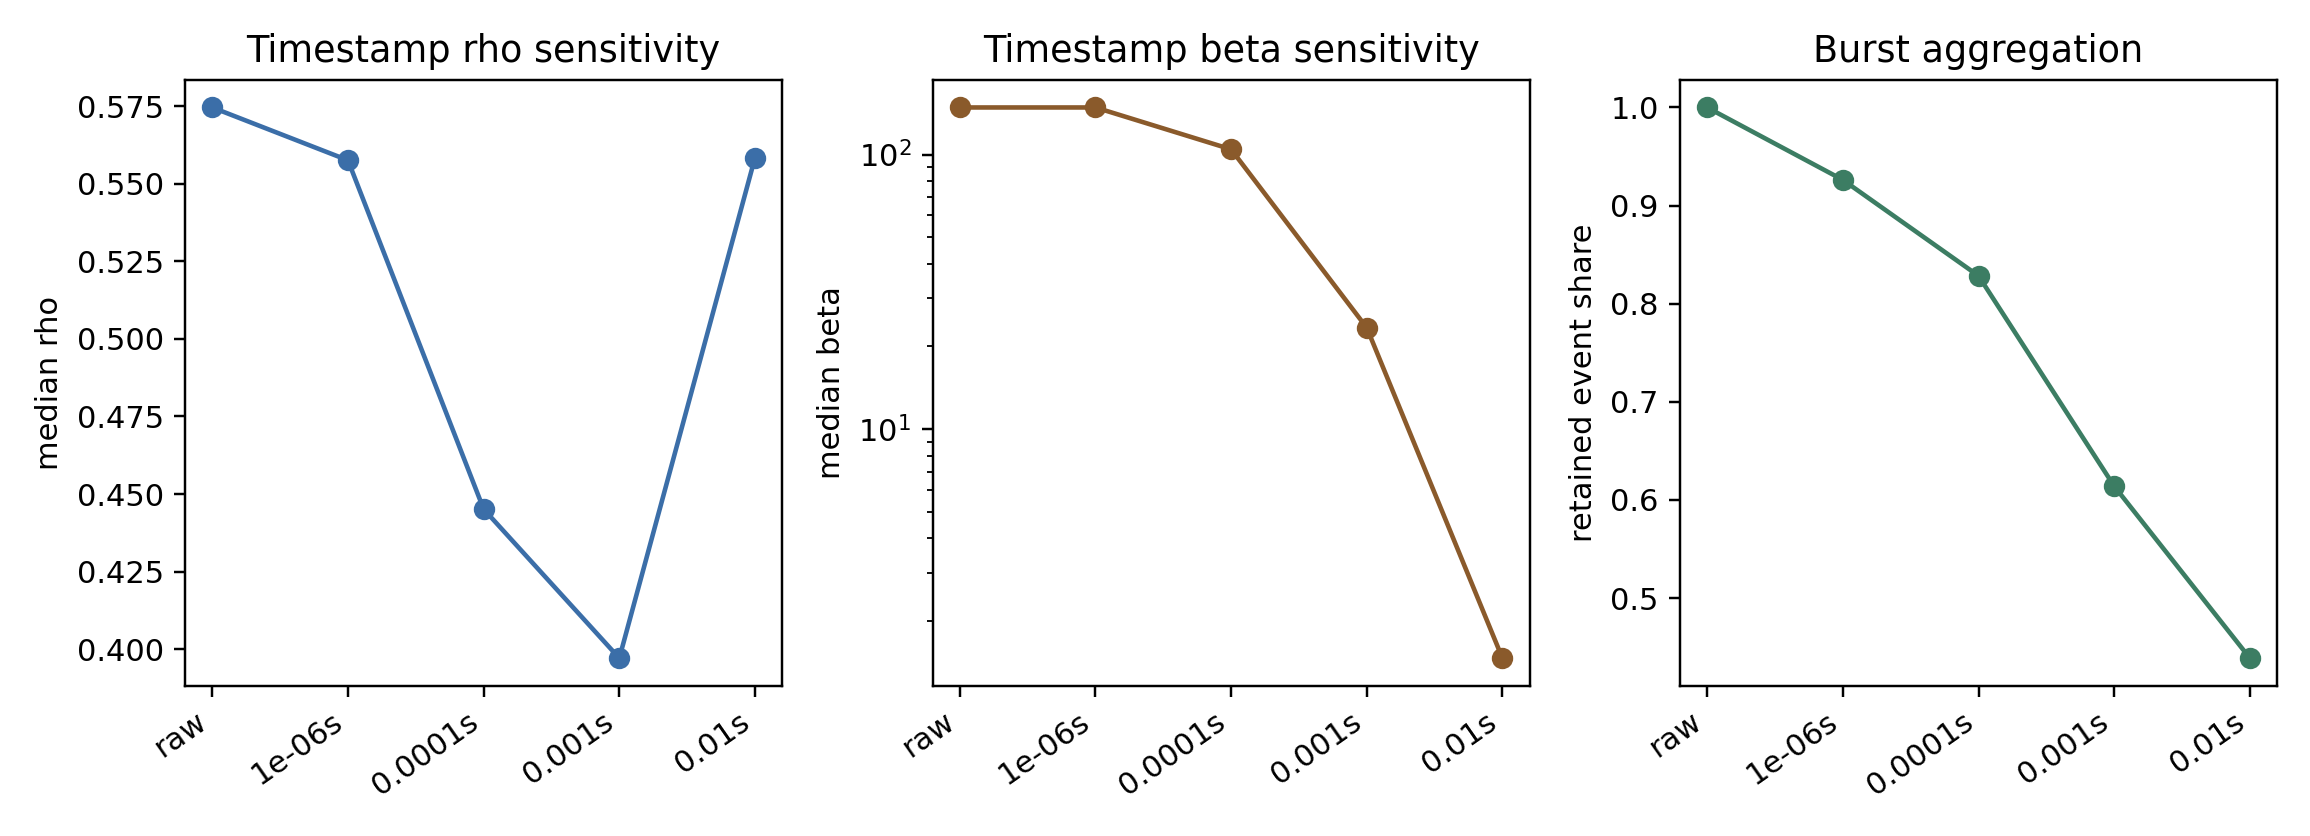
\includegraphics[width=.49\linewidth]{figures/lobster_timestamp_resolution_sensitivity.png}
\caption{Corrected public-data Hawkes diagnostics: event-type branching/decay
and timestamp-resolution sensitivity.}
\end{figure}

\begin{figure}[!htbp]
\centering
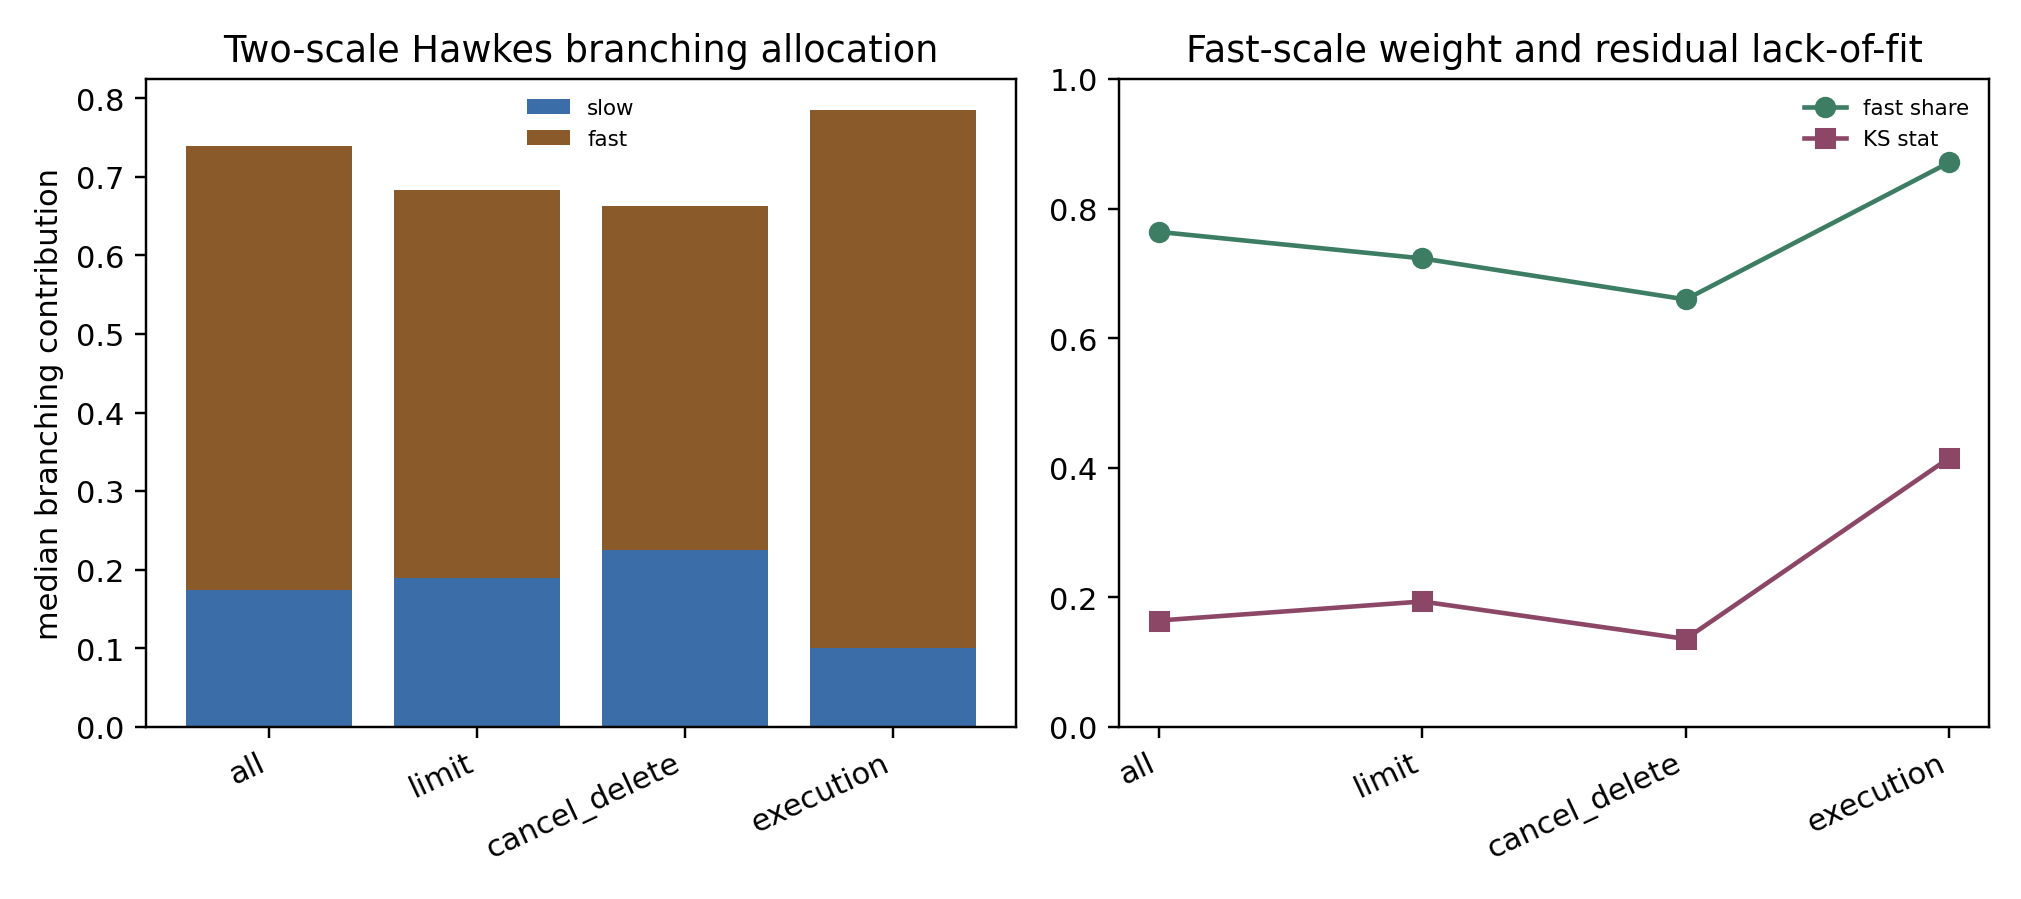
\includegraphics[width=.92\linewidth]{figures/lobster_hawkes_multiscale.png}
\caption{Fixed-beta two-scale public-data Hawkes diagnostics. The selected
fits concentrate excitation on the fast component, especially for execution
events, while residual tests still flag misspecification.}
\end{figure}

\begin{figure}[!htbp]
\centering
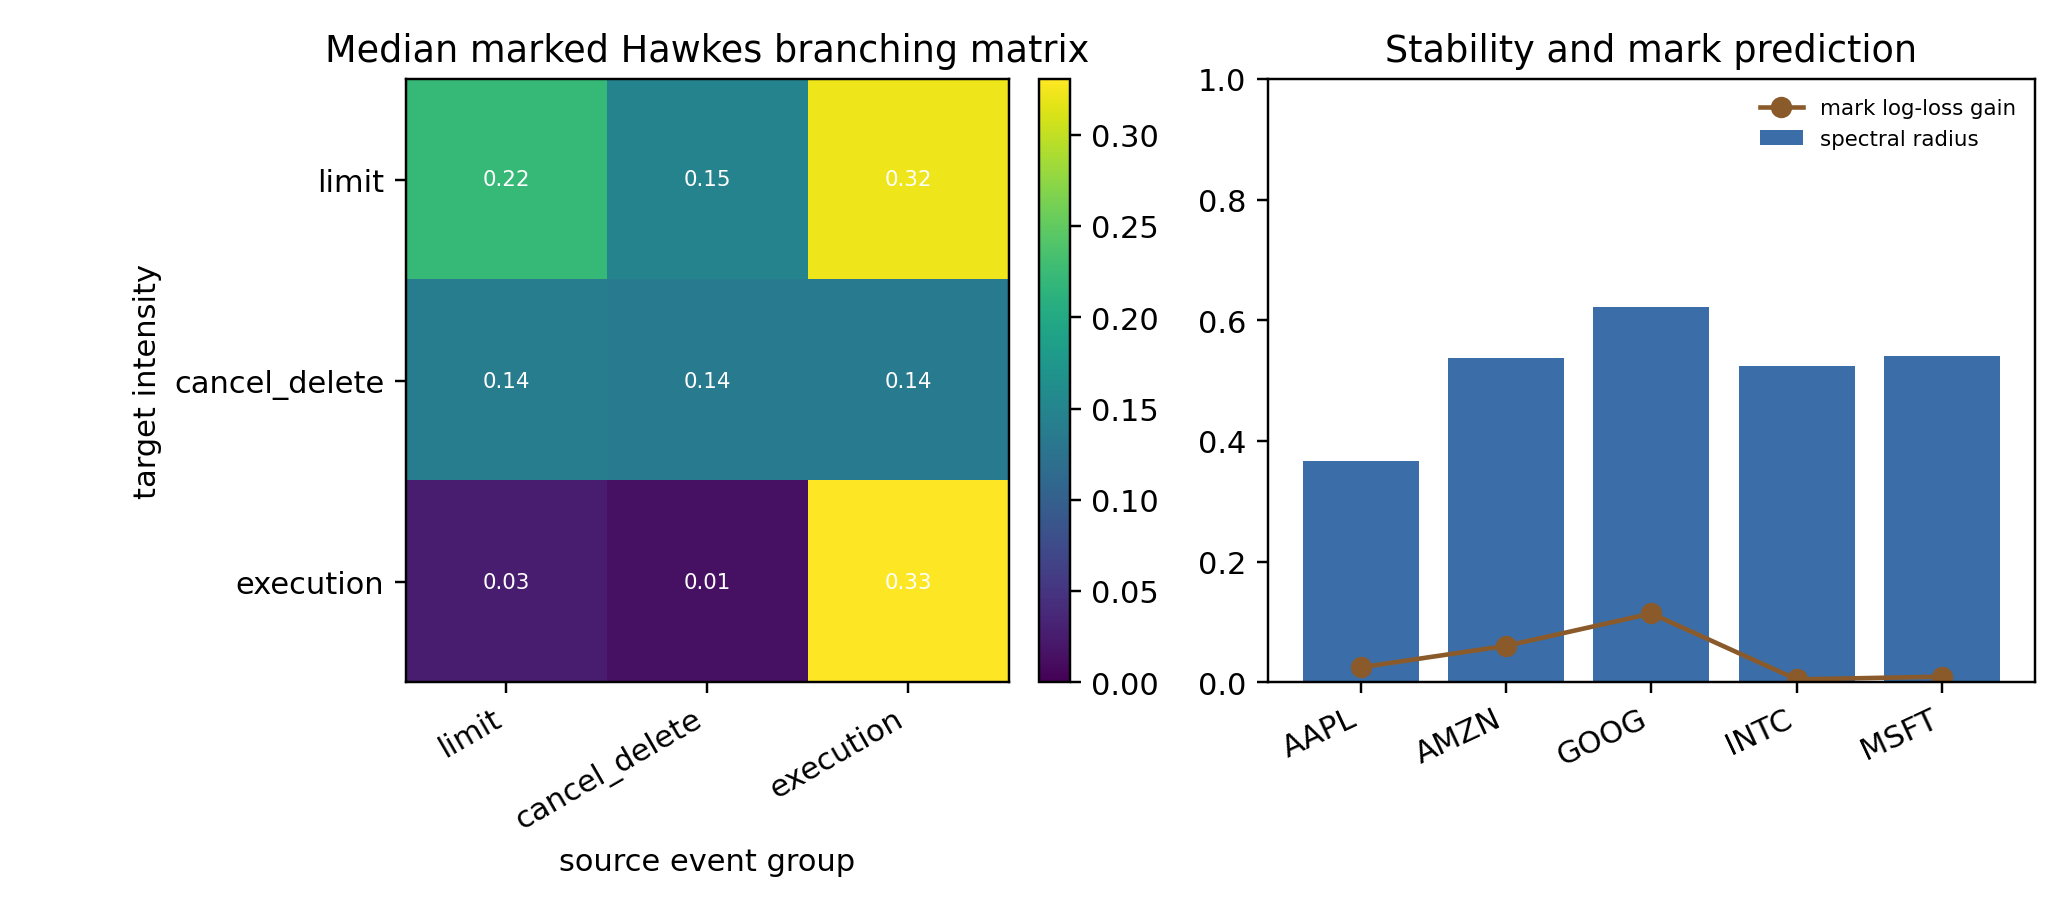
\includegraphics[width=.92\linewidth]{figures/lobster_marked_hawkes_multivariate.png}
\caption{Grouped marked multivariate Hawkes diagnostics on LOBSTER limit,
cancel/delete, and execution events. The fixed-beta fits estimate stable
branching matrices and improve conditional mark prediction, but residual tests
still point toward richer side, size, and multiscale calibration.}
\end{figure}

\begin{figure}[!htbp]
\centering
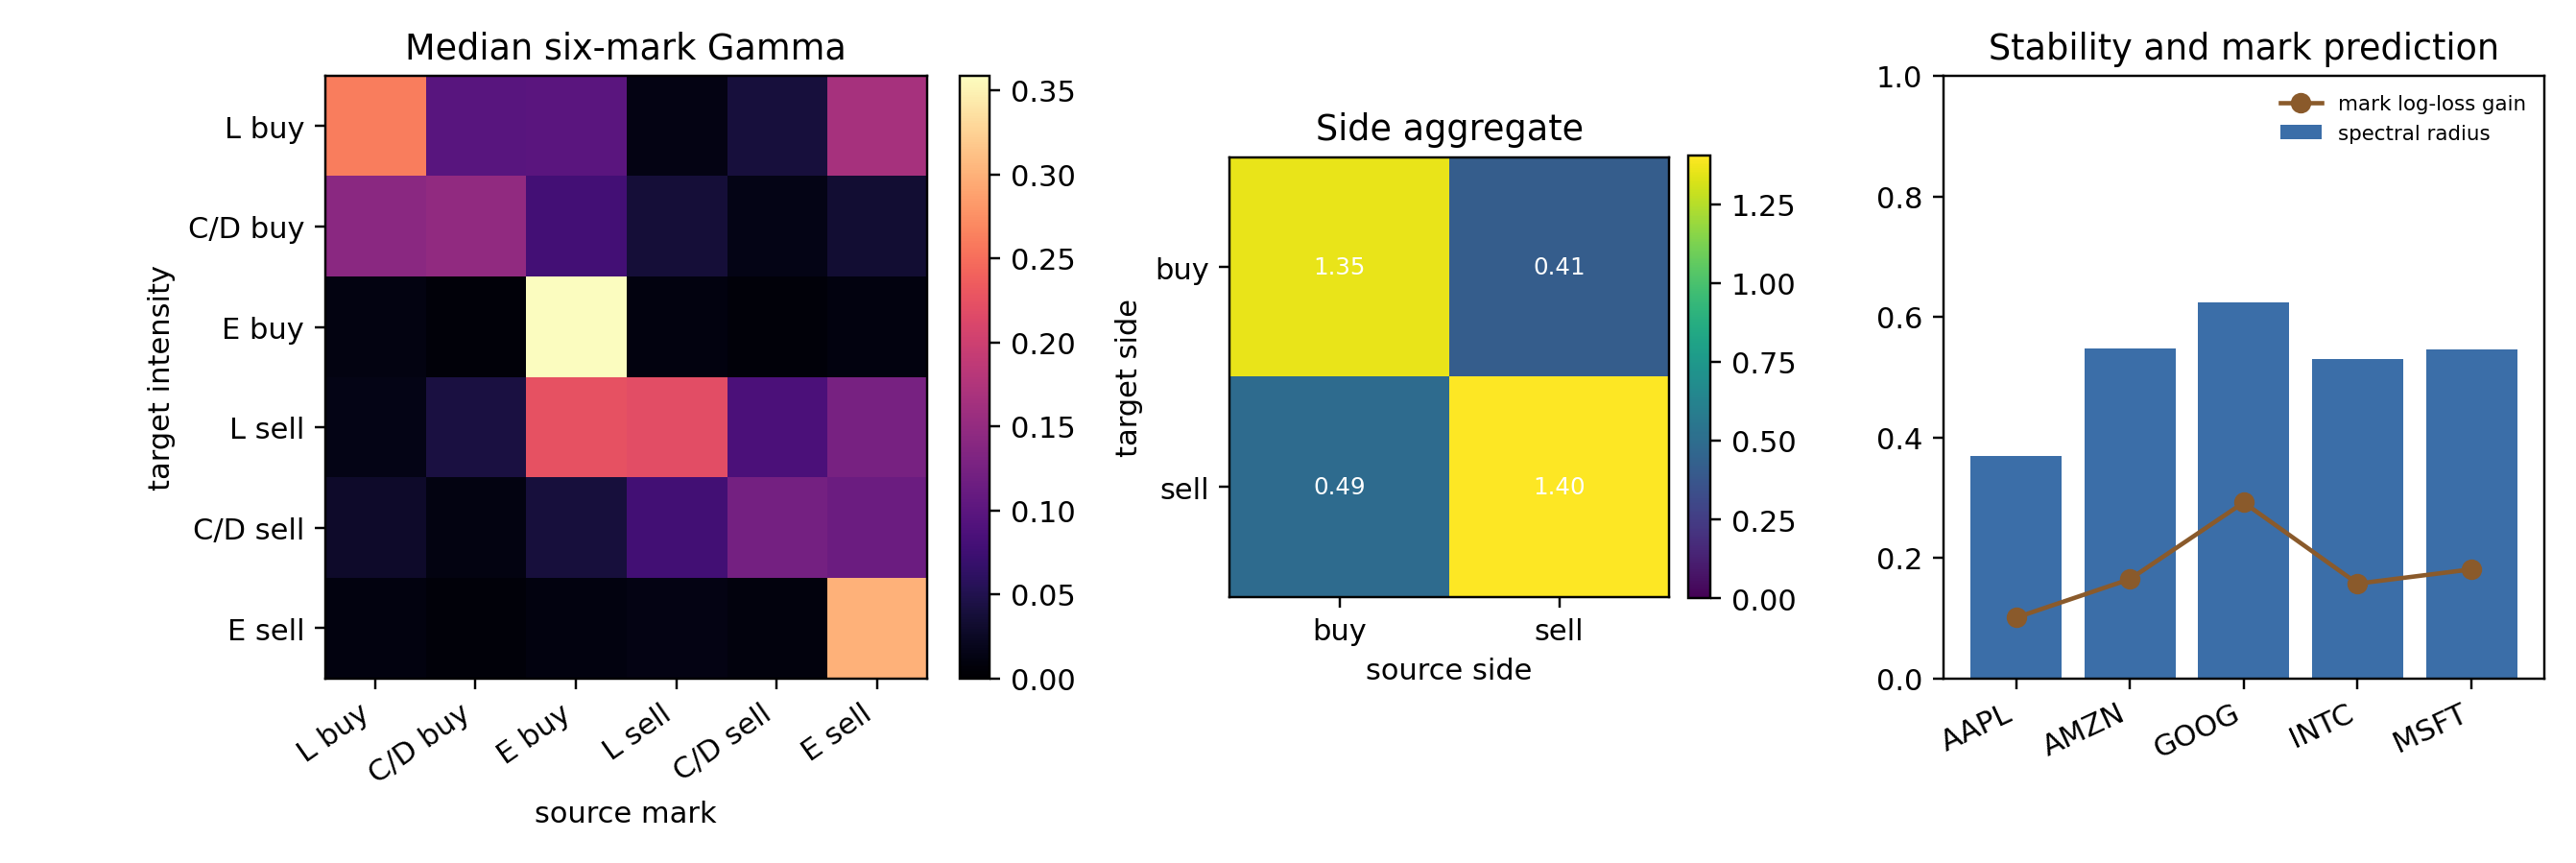
\includegraphics[width=.98\linewidth]{figures/lobster_side_marked_hawkes_multivariate.png}
\caption{Side-aware marked multivariate Hawkes diagnostics using LOBSTER
direction labels. The six-mark fits bring the empirical calibration object
closer to bid/ask robust control, while remaining fixed-decay and message-side
rather than queue-position or size-aware.}
\end{figure}

\begin{figure}[!htbp]
\centering
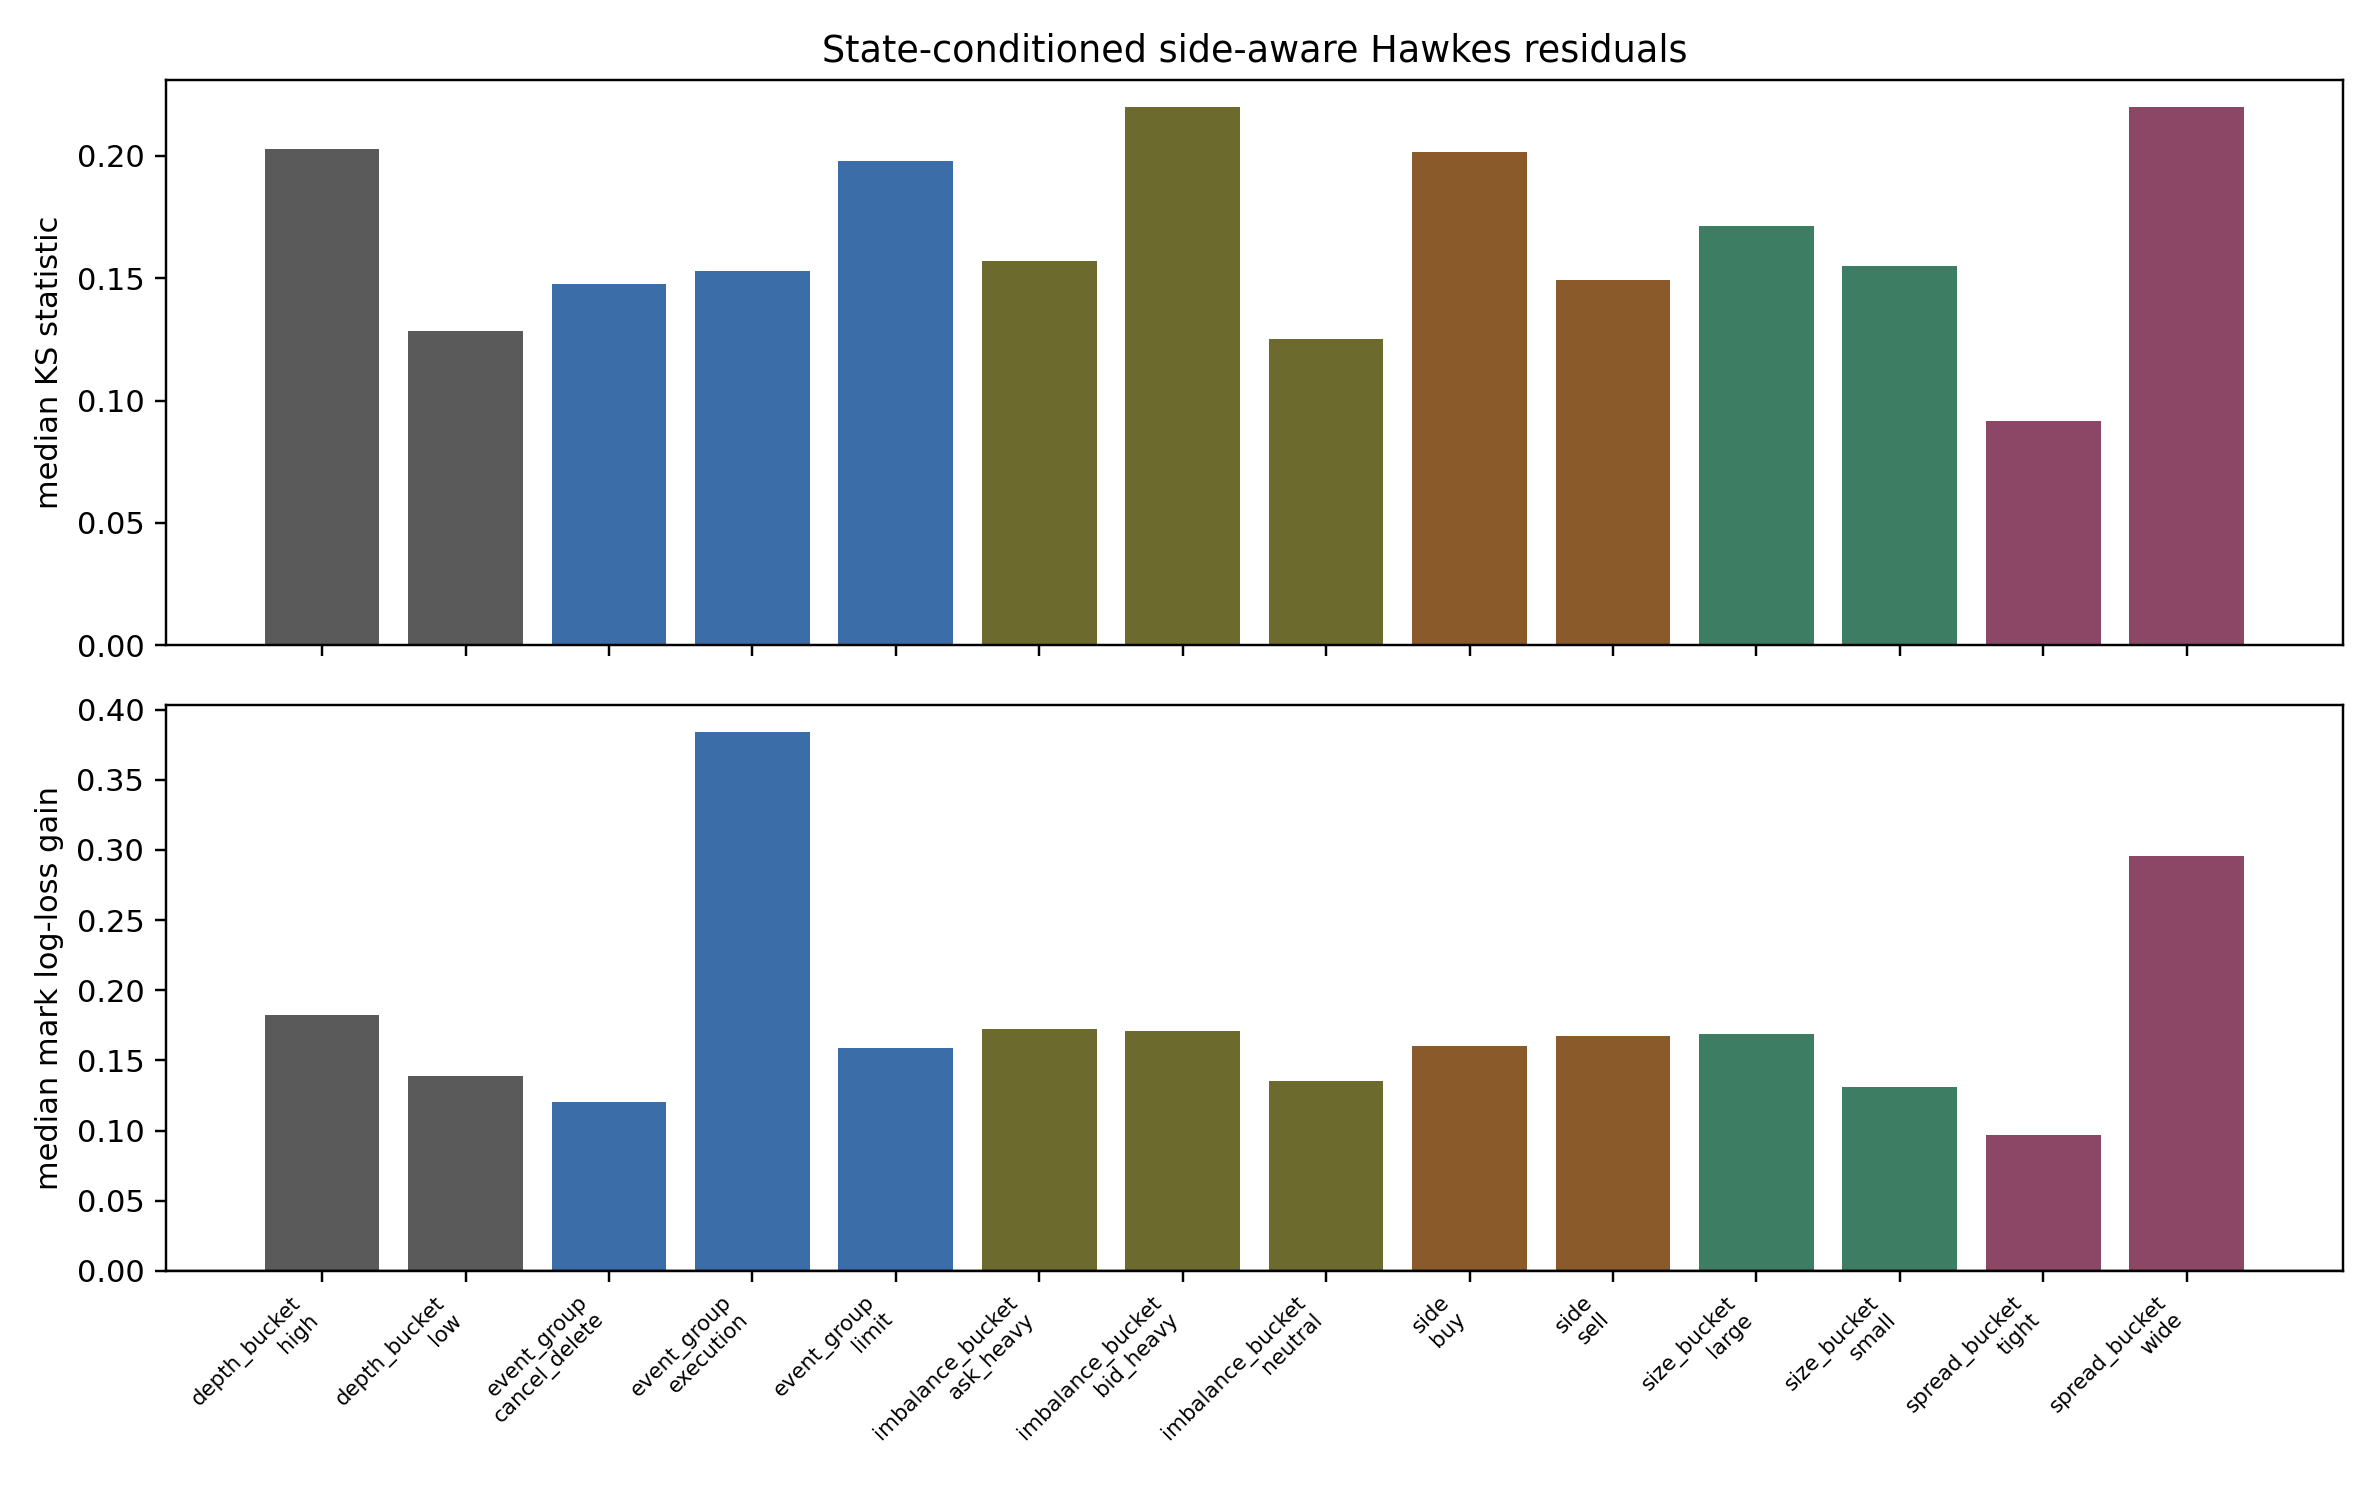
\includegraphics[width=.98\linewidth]{figures/lobster_side_marked_state_residuals.png}
\caption{State-conditioned residual diagnostics for the side-aware six-mark
Hawkes fit. Residual deviations and mark-prediction gains vary by spread,
depth, imbalance, and event-size bucket, so the public-data calibration is best
read as a diagnostic input rather than a complete structural law.}
\end{figure}

\FloatBarrier
\section{Limitations and Scope Conditions}

This paper develops a conditional multitype HJBI control link for the stated
exponential Hawkes model class. The argument combines compact truncated HJBI
verification under compact-PDMP DPP/comparison hypotheses, untruncated
Lyapunov stability with $p>1$ tail control, pairwise weighted comparison and
uniqueness in fixed-boundary $W_v$-weighted subclasses, local differentiability
of smooth interior quote optimizers, and a consolidated argument assembling
these pieces. It does not extend automatically to arbitrary state-dependent, learned,
multiscale, or power-law Hawkes kernels without rechecking the stated Lyapunov
and comparison assumptions. No-quote and active-adversary switches are treated
as nonsmooth control boundaries, not as classical optimizer derivatives.

The top-of-book, L1, displayed-depth, residual-volume priority-aware level-10,
deepest-public level-50, priority-sensitivity, and observable-reconstruction
LOBSTER checks should be read as public-data execution checks rather than
production execution claims, because hidden liquidity and anonymous initial
queue priority remain unobserved. Binance aggregate trades should be read as
event-clustering evidence rather than a queue-calibration source. These scope
conditions delimit the paper's claim: the reported results concern structural
Hawkes ambiguity, criticality amplification, and calibration fragility in the
stated Hawkes market-making experiments.

\begin{thebibliography}{99}
\raggedright
\bibitem{BacryMuzy2015} E. Bacry, I. Mastromatteo, and J.-F. Muzy. Hawkes
processes in finance. arXiv:1502.04592, 2015.
\bibitem{LawViens2019} B. Law and F. Viens. Market making under a weakly
consistent limit order book model. arXiv:1903.07222, 2019.
\bibitem{Kumar2024} P. Kumar. Deep Hawkes Process for High-Frequency Market
Making. Journal of Banking and Financial Technology, 2024. arXiv:2109.15110,
doi:10.1007/s42786-024-00049-8.
\bibitem{Raffaelli2026} D. Raffaelli, R. G. Cestari, D. Marazzina, and
S. Formentin. Forecasting Bitcoin price movements using multivariate Hawkes
processes and limit order book data. Decisions in Economics and Finance, 2026.
doi:10.1007/s10203-026-00570-z.
\bibitem{WangNoQuote2025} Z. Wang, C. Ventre, and M. Polukarov. Robust
Market Making: To Quote, or not To Quote. In ICAIF 2023: Proceedings of the
Fourth ACM International Conference on AI in Finance, pages 664--672, 2023.
doi:10.1145/3604237.3626858. arXiv:2508.16588, 2025.
\bibitem{WangHawkesARL2025} Z. Wang, C. Ventre, and M. Polukarov. ARL-Based
Multi-Action Market Making with Hawkes Processes and Variable Volatility. In
Proceedings of the 5th ACM International Conference on AI in Finance (ICAIF
2024), pages 437--444, 2024. doi:10.1145/3677052.3698695. arXiv:2508.16589,
2025.
\bibitem{LalorSwishchuk2025} L. Lalor and A. Swishchuk. Event-Based Limit
Order Book Simulation under a Neural Hawkes Process: Application in
Market-Making. arXiv:2502.17417, 2025.
\bibitem{GuoAttnLOB2023} H. Guo, J. Lin, and F. Huang. Market Making with Deep
Reinforcement Learning from Limit Order Books. In 2023 International Joint
Conference on Neural Networks (IJCNN), 2023. arXiv:2305.15821,
doi:10.1109/IJCNN54540.2023.10191123.
\bibitem{Jiang2025} J. Jiang, C. Yang, X. Wang, Z. Li, X. Huang, and B. Li.
Resolving Latency and Inventory Risk in Market Making with Reinforcement
Learning. arXiv:2505.12465, 2025.
\bibitem{Jain2025} K. Jain, N. Firoozye, J. Kochems, and P. Treleaven. An
Impulse Control Approach to Market Making in a Hawkes LOB Market.
arXiv:2510.26438, 2025.
\bibitem{ElKarmiSimulator2025} S. El Karmi. A Deterministic Limit Order Book
Simulator with Hawkes-Driven Order Flow. arXiv:2510.08085, 2025.
\bibitem{Noble2026} P. Noble, M. Rosenbaum, and S. Souilmi. Bridging the
Reality Gap in Limit Order Book Simulation. arXiv:2603.24137, 2026.
\bibitem{Kimura2026} A. Kimura. Extended State-dependent Hawkes Process for
Limit Order Books: Mathematical Foundation and the Reproduction of Volatility
Signature Plots. arXiv:2604.23961, 2026.
\bibitem{SzymanskiXu2025} G. Szymanski and W. Xu. Mean-Field Limits for
Nearly Unstable Hawkes Processes. arXiv:2501.11648, 2025.
\bibitem{ElKarmi2026} S. El Karmi. Scaling Limits of Bivariate
Nearly-Unstable Hawkes Processes and Applications to Rough Volatility.
arXiv:2605.03703, 2026.
\bibitem{Hardiman2013} S. J. Hardiman, N. Bercot, and J.-P. Bouchaud.
Critical reflexivity in financial markets: a Hawkes process analysis.
arXiv:1302.1405, 2013.
\bibitem{Ogata1988} Y. Ogata. Statistical models for earthquake occurrences
and residual analysis for point processes. Journal of the American Statistical
Association, 83(401):9--27, 1988.
\url{https://doi.org/10.1080/01621459.1988.10478560}.
\bibitem{CrandallIshiiLions1992} M. G. Crandall, H. Ishii, and P.-L. Lions.
User's guide to viscosity solutions of second order partial differential
equations. Bulletin of the American Mathematical Society, 27(1):1--67, 1992.
doi:10.1090/S0273-0979-1992-00266-5.
\bibitem{FlemingSoner2006} W. H. Fleming and H. M. Soner. Controlled Markov
Processes and Viscosity Solutions. 2nd ed., Springer, 2006.
doi:10.1007/0-387-31071-1.
\bibitem{Davis1993} M. H. A. Davis. Markov Models and Optimization. Chapman
\& Hall, 1993. ISBN 9780412314100.
\end{thebibliography}

\end{document}
